\chapter{Subjective Timbre Evaluation}
\label{chap:TimbreEvaluation}
	\todo{Come up with a better name for this chapter.}

\section{Introduction}
\label{sec:TimbreEvaluation-Introduction}
	In order to manipulate the perceptual characteristics of a sound it is necessary to know the relationships between
	low level audio features and semantic descriptions. In Chapter \ref{chap:Timbre} several different methods for
	obtaining this information were discussed.  In this chapter a new method of collecting semantically annotated audio
	feature data is presented (Section \ref{sec:TimbreEvaluation-DAWBasedTimbreEvaluation}). Data gathered using this
	method is then analysed, producing a list of semantic descriptors and the low level audio features which contribute
	to them (Section \ref{sec:TimbreEvaluation-Analysis}).

\section{Production Environment Timbre Evaluation} % this name will probably change
\label{sec:TimbreEvaluation-DAWBasedTimbreEvaluation}
	The perceptual listening test methodologies discussed in Section \ref{sec:Timbre-ListeningTests} rely on the
	participants performing a certain set of tasks. While this structure helps to reduce the number of variables in an
	experiment, it does not necessarily reflect the way audio is treated in a production environment.

	A new methodology has been developed in which the analysis of timbre is introduced into a typical music production
	workflow, causing minimal interruption to the producer. This methodology aims to answer the question "What terms do
	music producers use to describe the timbral transforms, they apply to audio, during the creation of music?". 

	This section will detail a typical production workflow is and how semantic information can be gathered.

	\subsection{Music Production Workflow}
	\label{sec:TimbreEvaluation-DAWBasedTimbreEvaluation-Workflow}
		\todo{Find some references for this section. Probably mixing engineers handbook or something.}

		The music production workflow has four main stages:

		\begin{itemize}
			\item Recording
			\item Editing
			\item Mixing
			\item Mastering
		\end{itemize}

		At every stage of this process semantic descriptors are often used to communicate the desired timbral
		qualities of the audio. For instance, one my ask that a certain microphone be used because of the `warmth'
		it adds to the recorded sound. During the mixing and mastering stages audio processing effects are applied
		to shape the timbre further. These stages will be the focus of this section as the aim of this thesis is
		to improve the intuitiveness of these effects.

		Historically, audio production required the use of several pieces of electronic hardware, including
		microphones, a mixing console, audio processing effects and a recording device. Modern music production
		techniques utilise Digital Audio Workstation (DAW) software. This software performs the tasks of many
		pieces of hardware, enabling users to record, edit and mix multiple tracks of audio using a computer. 
		
	\subsection{Analysis of Timbre Inside the DAW}
	\label{sec:TimbreEvaluation-DAWBasedTimbreEvaluation-InDAW}
		An ideal way to collect timbral information during music production would be to have the DAW analyse the
		audio tracks used and production techniques applied. Information which could be gathered directly from the
		DAW, with no extra input from the user, includes:

		\begin{itemize}
			\item Information about the audio processing chain:
			\begin{itemize}
				\item The effects applied to each track.
				\item The order in which these effects are applied.
				\item The parameter settings of these effects.
			\end{itemize}
			\item Features of the audio signal at every stage in the processing chain.
		\end{itemize}

		Additional information can be gathered by prompting the user for input:

		\begin{itemize}
			\item The genre of music being produced.
			\item The content of the separate audio tracks (what instruments etc.).
			\item Semantic terms which describe the timbral transforms applied by each audio
			      effect.
		\end{itemize}

		Achieving this would require the creation of a new DAW. This would be impractical for the current research.
		DAWs are comprehensive software packages which perform many more tasks than the application of audio
		effects (project management, audio editing functionality etc.). A lot of effort would be expended in
		implementing these features before any timbral data could be collected. Music producers also tend to have
		a preferred DAW with which they work most fluidly. Convincing producers to use a new DAW, for the purposes
		of research, would be a difficult task.

		Third party developers can produce extensions to DAWs known as plug-ins. Plug-Ins provide additional audio
		processing functionality to the DAW environment. They can optionally expose their own parameters which
		users can adjust to achieve their desired effect. There are several different formats in which audio
		plug-ins can be distributed (VST, AU etc.). Most of the commonly used DAWs support plug-ins in one or more
		of these formats.

		Audio plug-ins provide a good platform to allow producers to provide semantic terms and audio feature
		information from within their preferred DAW. As part of this research a suite of audio plug-ins which
		extract this information have been developed. They have been released under the title Semantic Audio
		Feature Extraction (SAFE) Plug-Ins.

	\subsection{SAFE Plug-Ins}
	\label{sec:TimbreEvaluation-DAWBasedTimbreEvaluation-SAFE}
		The SAFE plug-ins consist of four commonly used audio effects: Equaliser, Distortion, Compressor and
		Reverb. As part of the plug-ins's interface, the user has the option to save semantic terms. The interface
		for the SAFE Distortion is shown in Figure \ref{fig:SAFE-Distortion}. Upon saving terms the plug-in will
		analyse the audio at its inputs and outputs. When the analysis is completed the results are stored,
		containing:

		\begin{itemize}
			\item The users semantic description of the transform.
			\item The plug-in's current parameter settings.
			\item The features of the audio before and after processing.
			\item Some additional data about the user and the track being worked on.
			\begin{itemize}
				\item The genre.
				\item The instrument.
				\item The users age.
				\item The users location.
				\item The users primary language.
				\item The number of year experience the user has in music production.
			\end{itemize}
		\end{itemize}

		\begin{figure}[h!]
			\centering
			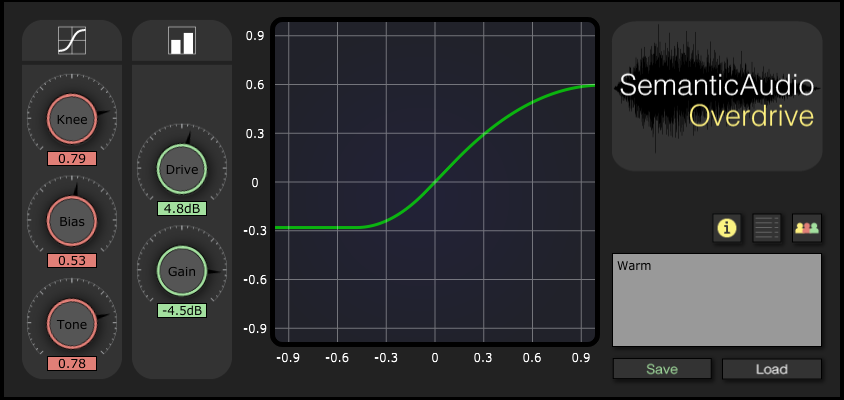
\includegraphics[width=0.8\textwidth]{chapter4/Images/SAFEDistortion.png}
			\caption{The interface for the SAFE distortion plug-in.}
			\label{fig:SAFE-Distortion}
		\end{figure}

		In total, the SAFE plug-ins analyse five seconds of audio both before and after processing. The audio is
		analysed in frames of 4096 samples using the LibXtract software library \citep{bullock2007libxtract},
		calculating 80 different audio features for each frame. These features are split into five groups as
		follows:

		\begin{itemize}
			\item {\bf{Temporal Features:}} Features calculated from the temporal representation of the signal.
			\begin{itemize}
				\item Signal Mean, Signal Variance, Signal Standard Deviation, RMS Amplitude and Zero
					Crossing Rate.
			\end{itemize}
			\item {\bf{Spectral Features:}} Features calculated from the DFT of the signal.
			\begin{itemize}
				\item Spectral Centroid, Spectral Spread, Spectral Standard Deviation, Spectral Skewness,
				      Spectral Kurtosis, Jensen Irregularity, Krimphoff Irregularity, $f_{0}$, Spectral
				      Smoothness, Spectral Roll Off, Spectral Flatness, Tonality, Spectral Crest and
				      Spectral Slope
			\end{itemize}
			\item {\bf{Peak Spectral Features:}} Features calculated from the spectral partials of the signal.
			\begin{itemize}
				\item Peak Spectral Centroid, Peak Spectral Spread, Peak Spectral Standard Deviation, Peak
					Spectral Skewness, Peak Spectral Kurtosis, Peak Jensen Irregularity, Peak Krimphoff
					Irregularity, Peak Tristimuli and Inharmonicity.
			\end{itemize}
			\item {\bf{Harmonic Spectral Features:}} Features calculated from the harmonic partials of the
			      signal.
			\begin{itemize}
				\item Harmonic Spectral Centroid, Harmonic Spectral Spread, Harmonic Spectral Standard
					Deviation, Harmonic Spectral Skewness, Harmonic Spectral Kurtosis, Harmonic Jensen
					Irregularity, Harmonic Krimphoff Irregularity, Tristimuli, Noisiness and Odd to
					Even Harmonic Ratio.
			\end{itemize}
			\item {\bf{Bark Coefficient 0-24:}} The 25 bark band coefficients.
			\item {\bf{MFCC 0-12:}} The 13 MFCCs.
		\end{itemize}

		One disadvantage in using plug-ins is that they cannot gather information about the processing chain they
		may be a part of. The timbral transform the user is describing may be the result of several effects working
		together. This can be mitigated somewhat by asking users to describe only the effect the plug-in in
		question is providing.

		The SAFE plug-ins suffer from the same issues other distributed tests do. The researcher forfeits control
		over the listening environment in order to gather results from a much larger sample of people. In fact they
		provide even lest control than methodologies like that used in the Social EQ project
		\citep{cartwright2013socialeq} in that the choice of audio samples being used is decided by the test
		subject. 

	\subsection{SAFE Ontology}
	\label{sec:TimbreEvaluation-DAWBasedTimbreEvaluation-SAFEOntology}
		\note{Really not sure how well this fits in here. Do we needs a section explaining RDF and such? Where
		would that go?}

		The data collected using the SAFE plug-ins is stored as RDF triples using the SAFE ontology.  The SAFE
		Ontology was designed to describe the semantics relating to the application of an audio effect and the
		statistical audio features of the signals involved. It acts as an extension to the Audio Effects Ontology
		\citep{wilmering2013the}, introducing additional concepts for the description of semantic data.  This
		additional data can be separated into three groups:

		\begin{itemize}
			\item Metadata describing the application of the effect.
			\item Audio feature data for the input and output signals.
			\item Provenance of the data.
		\end{itemize}

		Each entry in the SAFE dataset is described using the \emph{studio:Transform} concept, applying some
		semantic transform to a set of input signals to produce a set of output signals. The structure of this data
		is shown in Figure \ref{fig:TransformGraph}.

		\begin{figure}[h!]
			\centering
			\begin{tikzpicture}[->,>=stealth',node distance=3cm,every node/.style={scale=0.75}]
				\tikzstyle{object} = [style=ellipse]

				\node[object, fill=blue] (transform) {studio:Transform};
				\node[object, fill=green] (signal) [below left of=transform] {mo:Signal};
				\node[object, fill=orange] (descriptor) [above of=transform] {safe:DescriptorItem};
				\node[object, fill=orange] (metadata) [below right of=transform] {safe:MetadataItem};
				\node[object, fill=pink] (device) [above right=1.3cm and 0.6cm of transform] {afx:Device};
				\node[object, fill=pink] (state) [above left=1.3cm and 0.6cm of transform] {afx:State};
				\node[object, fill=gray] (harsh) [above=1cm of descriptor] {"Harsh"};

				\path (transform) edge [bend left] node [right, overlay] {prov:used} (signal)
				      edge [bend right] node [left, overlay] {prov:generated} (signal)
				      edge node [right, overlay] {safe:descriptor} (descriptor)
				      edge [bend left] node [right, overlay] {safe:metadata} (metadata)
				      edge [bend right] node [right, overlay] {studio:effect} (device)
				      edge [bend left] node [left, overlay] {afx:state} (state)
				      (signal) edge [bend right] node [below, overlay] {safe:metadata} (metadata)
				      (descriptor) edge node [right, overlay] {rdfs:comment} (harsh);
			\end{tikzpicture}
			\caption{The structure used to describe the application of an audio effect.}
			\label{fig:TransformGraph}
		\end{figure}

		Here, users provide a term, or series of terms, to describe the transform applied by the audio effect in
		its current state. This should describe the perceived difference between the output and input signals. In
		the SAFE Ontology this is modelled through the \emph{safe:DescriptorItem} concept which provides a semantic
		description for each transform. Metadata items are used to provide details about the application domain of
		the effect, where each metadata item describes one property of an object, the property being identified
		using an \emph{rdfs:label} and the description provided using an \emph{rdfs:comment}. Each object described
		by a metadata item has its own set of properties, ``genre'' and ``instrument'' metadata tags for example,
		describe an audio signal, while ``location'' metadata tags describe a transform.

		The analysis of audio signals is described using the concept \emph{safe:FeatureExtractionTransform},
		similar to a \emph{studio:Transform} but taking an audio signal as input and producing feature values at
		the output, as shown in Figure \ref{fig:ExtractionGraph}.

		\begin{figure}[h!]
			\centering
			\begin{tikzpicture}[->,>=stealth',node distance=3cm,every node/.style={scale=0.75}]
				\tikzstyle{object} = [style=ellipse]

				\node[object, fill=orange] (extraction) {safe:FeatureExtractionTransform};
				\node[object, fill=gray] (feature) [above of=extraction] {"Spectral Centroid"};
				\node[object, fill=gray] (frameSize) [above left of=extraction] {"4096"};
				\node[object, fill=gray] (stepSize) [above right of=extraction] {"1024"};
				\node[object, fill=green] (signal) [below left of=extraction] {mo:Signal};
				\node[object, fill=purple] (event) [below right of=extraction] {event:Event};
				\node[object, fill=yellow] (interval) [below=1cm of signal] {tl:Interval};
				\node[object, fill=yellow] (instant) [below=1cm of event] {tl:Instant};
				\node[object, fill=yellow] (timeline) [below right of=interval] {tl:TimeLine};
				\node[object, fill=gray] (value) [below right=0.2cm and 0.6cm of event] {"2543.4"};
				\node[object, fill=gray] (time) [below right=0.2cm and 0.6cm of instant] {"4048"};

				\path (extraction) edge [bend left] node [left, overlay] {safe:frameSize} (frameSize)
				      edge [bend right] node [right, overlay] {safe:stepSize} (stepSize)
				      edge node [right, overlay] {rdfs:label} (feature)
				      edge [bend right] node [left, overlay] {prov:used} (signal)
				      (signal) edge node [left, overlay] {mo:time} (interval)
				      (event) edge node [left, overlay] {event:time} (instant)
				      edge [bend right] node [right, overlay] {prov:wasGeneratedBy} (extraction)
				      edge node [above right, overlay] {af:feature} (value)
				      (interval) edge [bend right] node [left, overlay] {tl:onTimeLine} (timeline)
				      (instant) edge [bend left] node [right, overlay] {tl:onTimeLine} (timeline)
				      edge node [above right, overlay] {tl:at} (time);

			\end{tikzpicture}
			\caption{The structure used to describe the features of an audio signal.}
			\label{fig:ExtractionGraph}
		\end{figure}

		Here, The SAFE Ontology makes extensive use of the Provenance Ontology to identify the origins of the data.
		Each element of data constitutes a \emph{prov:Entity} which was generated by a \emph{prov:Activity}. These
		\emph{prov:Activity} nodes are in turn associated with a \emph{prov:Agent} identifying the way that the
		data was produced.

		When using the SAFE plug-ins, users are required to provide a descriptor for a transform, meaning that
		every \emph{safe:DescriptorItem} node in the dataset is attributed to a particular user. Conversely, the
		metadata fields are not mandatory. In situations where a user has not filled in certain metadata fields
		their values can be predicted on the server using supervised machine learning. Using the Provenance
		Ontology, each metadata entity can be attributed to a particular agent, allowing it to understood as human
		or machine labelled. This allows queries on the dataset to request only the more reliable user-labeled
		data, or for example, compare data produced using different classification algorithms.

		The Provenance Ontology is also used to describe the algorithms that produce audio feature data. Each
		\emph{safe:FeatureExtractionTransform} node is a \emph{prov:Activity} which can be associated with a
		particular implementation of the algorithm it uses (e.g. the LibXtract \citep{bullock2007libxtract}
		spectral centroid function). Say a discrepancy was found between two implementations of a given feature
		extraction algorithm, the provenance data allows queries to filter results to remove those generated using
		an earlier or incompatible implementation. Further use of provenance describes the role of a user in the
		application of a transform. Storage of this data allows the simple retrieval of all transforms associated
		with a particular user, allowing users to maintain personal libraries of semantic presets amongst the
		entire SAFE dataset.

\section{Analysis}
\label{sec:TimbreEvaluation-Analysis}
	In this section the data collected using the SAFE plug-ins is analysed. For the purposes of this study only the
	data from the distortion and equaliser plug-ins is used as these effects best represent the timbral transforms
	which can be applied using harmonic excitation. The distortion showing the effects of introducing new spectral
	content and the equaliser showing the effects of manipulating the existing spectral content.

	Firstly, the terms used to describe transforms using each plug-in are investigated (Section
	\ref{sec:TimbreEvaluation-Analysis-TermUsage}). This provides insight into the language used to describe audio in
	the production environment, also showing what terms are shared across processing techniques and those which are
	reserved for particular effect. Secondly, clustering techniques are used in order to group these terms into those
	which describe similar audio signals / transforms, finding terms which are synonymous when used to describe
	timbre (Section \ref{sec:TimbreEvaluation-Analysis-TermClustering}). Finally, timbre spaces are constructed using
	PCA in order to find the most salient audio features which contribute to the differences in timbral description.

	\subsection{Term Usage}
	\label{sec:TimbreEvaluation-Analysis-TermUsage}
		Tables \ref{tab:DistortionTerms} and \ref{tab:EqualiserTerms} show the most commonly used terms used to
		describe transforms applied by the distortion and equaliser respectively.

		\begin{table}[h!]
			\centering
			\begin{tabular}{|c|c|}
				\hline
				\bf{Term} & \bf{Frequency} \tabularnewline
				\hline
				\hline
				warm & 21 \tabularnewline
				\hline
				crunch & 16 \tabularnewline
				\hline
				crunchy & 10 \tabularnewline
				\hline
				fuzz & 9 \tabularnewline
				\hline
				creamy & 6 \tabularnewline
				\hline
			\end{tabular}
			\qquad
			\begin{tabular}{|c|c|}
				\hline
				\bf{Term} & \bf{Frequency} \tabularnewline
				\hline
				\hline
				fuzzy & 6 \tabularnewline
				\hline
				bright & 5 \tabularnewline
				\hline
				harsh & 4 \tabularnewline
				\hline
				raspy & 4 \tabularnewline
				\hline
				smooth & 3 \tabularnewline
				\hline
			\end{tabular}
			\caption{Most commonly used terms from the distortion.}
			\label{tab:DistortionTerms}
		\end{table}

		\begin{table}[h!]
			\centering
			\begin{tabular}{|c|c|}
				\hline
				\bf{Term} & \bf{Frequency} \tabularnewline
				\hline
				\hline
				warm & 437 \tabularnewline
				\hline
				bright & 408 \tabularnewline
				\hline
				clear & 17 \tabularnewline
				\hline
				thin & 11 \tabularnewline
				\hline
				airy & 9 \tabularnewline
				\hline
			\end{tabular}
			\qquad
			\begin{tabular}{|c|c|}
				\hline
				\bf{Term} & \bf{Frequency} \tabularnewline
				\hline
				\hline
				boomy & 8 \tabularnewline
				\hline
				air & 7 \tabularnewline
				\hline
				brighter & 6 \tabularnewline
				\hline
				deep & 6 \tabularnewline
				\hline
				full & 6 \tabularnewline
				\hline
			\end{tabular}
			\qquad
			\begin{tabular}{|c|c|}
				\hline
				\bf{Term} & \bf{Frequency} \tabularnewline
				\hline
				\hline
				tinny & 6 \tabularnewline
				\hline
				muddy & 5 \tabularnewline
				\hline
				boxy & 4 \tabularnewline
				\hline
				harsh & 4 \tabularnewline
				\hline
				box & 3 \tabularnewline
				\hline
			\end{tabular}
			\caption{Most commonly used terms from the equaliser.}
			\label{tab:EqualiserTerms}
		\end{table}

		\note
		{
			Should we mention how `warm' and `bright' from the EQ have so many instances because they were part
			of an experiment?
		}

		The terms `warm' and `bright' have been used to describe transforms applied using both the distortion and
		the equaliser effects, suggesting that the timbral characteristics these terms describe can be manipulated
		using either effect. Other descriptors are only used to describe transforms applied using a specific
		effect, suggesting that a unique property of that effect produces tat timbral result. For example the term
		`crunch' is only used to in relation to the distortion effect.

		Several descriptors in the dataset are derived from the same root word with the addition of suffixes such
		as `y' or `er' (e.g. `crunch' and `crunchy' or `bright' and `brighter'). It is assumed that the addition of
		such suffixes has no effect over how a term is used to describe timbre. As such a stemming algorithm
		\citep{porter1980an} is used in order to reduce all descriptors in the dataset to their root words.
		Additional processing is required after stemming so that all descriptors with the same root can be
		combined.  The Porter stemming algorithm replaces the letter y at the end of a word with the letter i, for
		this analysis these tailing i's are removed so that terms such as `fuzz' and `fuzzy' are reduced to the
		same root. In some cases the output after this  must be further reduced, for example the term `muddy' is
		reduced to `mudd' which must have the tailing d removed to give the correct root `mud'.

		After stemming we are left with eight descriptors from the distortion (`warm', `crunch', `fuzz', `cream',
		`bright', `harsh', `rasp' and `smooth') and twelve descriptors from the equaliser (`warm', `bright',
		`clear', `thin', `air', `boom', `deep', `full', `tin', `mud', `box' and `harsh').

	\subsection{Term Clustering}
	\label{sec:TimbreEvaluation-Analysis-TermClustering}
		Each of the terms arrived at, after stemming, in Section \ref{sec:TimbreEvaluation-Analysis-TermClustering}
		can be described by their position in a multi dimensional audio feature space. Each dimension of this space
		corresponds to one of the audio features extracted by the SAFE plug-ins. The coordinates of each term are
		calculated as the mean audio features across each transform described by that term. For each audio effect
		two separate feature spaces are constructed, one in which a terms coordinates are calculated from the audio
		features of the processed signal and the other in which they are calculated from the difference between
		features of the output and input signal. These two spaces can be compared to determine whether certain
		descriptors are mostly used to describe a transform (e.g. an increase in inharmonicity) or are used to
		describe an output signal (e.g. a signal with a spectral centroid between 4 and 8kHz).

		To identify groups of semantically similar descriptors hierarchical clustering is applied to these feature
		spaces. Prior to clustering, each dimension of the feature space is standardised, to mitigate any effect
		the range of a particular audio feature might have on the clustering. Clusters are determined using the
		ward linkage criterion in order to minimise the variance within each cluster.

		Figure \ref{fig:DistortionClusters} shows dendrograms illustrating the clustering of terms for the
		distortion features spaces. The clusters identified are similar for both the processed features
		(\ref{fig:DistortionProcessedClusters}) and the feature differences
		(\ref{fig:DistortionDifferenceClusters}), the cluster containing `harsh' and `bright' being the most
		distant from that containing `warm', `cream' and `fuzz' and the term `crunch' siting in a cluster separate
		from the majority of the other terms. This leads to the formation of three distinct timbral groups used to
		describe the application of distortion (`warmth', `brightness' and `crunchiness'). 

		\begin{figure}[h!]
			\centering
			\subfloat[Processed Features]
			{
				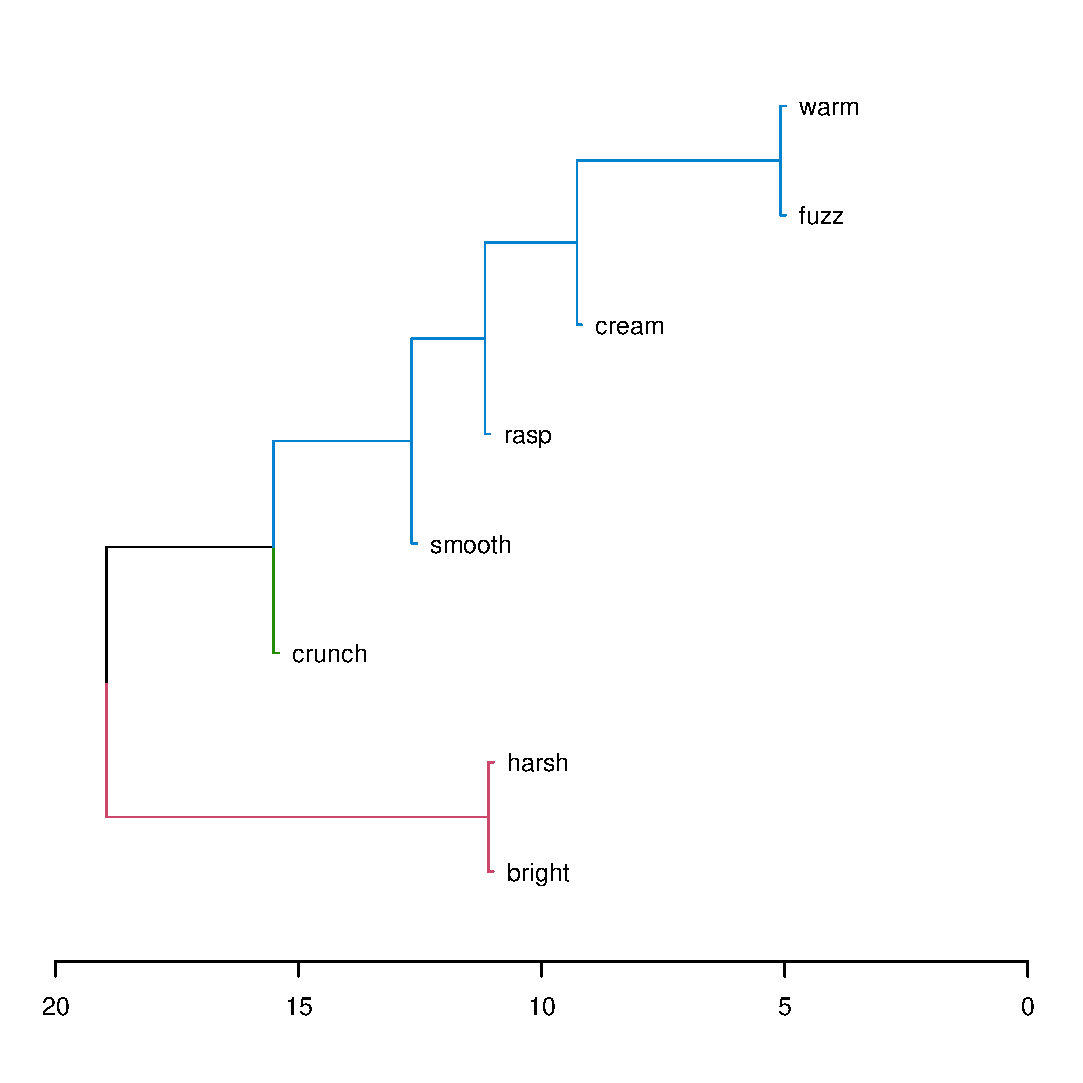
\includegraphics[width=0.45\textwidth]{chapter4/Images/DistortionProcessedClusters.eps}
				\label{fig:DistortionProcessedClusters}
			}
			\qquad
			\subfloat[Feature Differences]
			{
				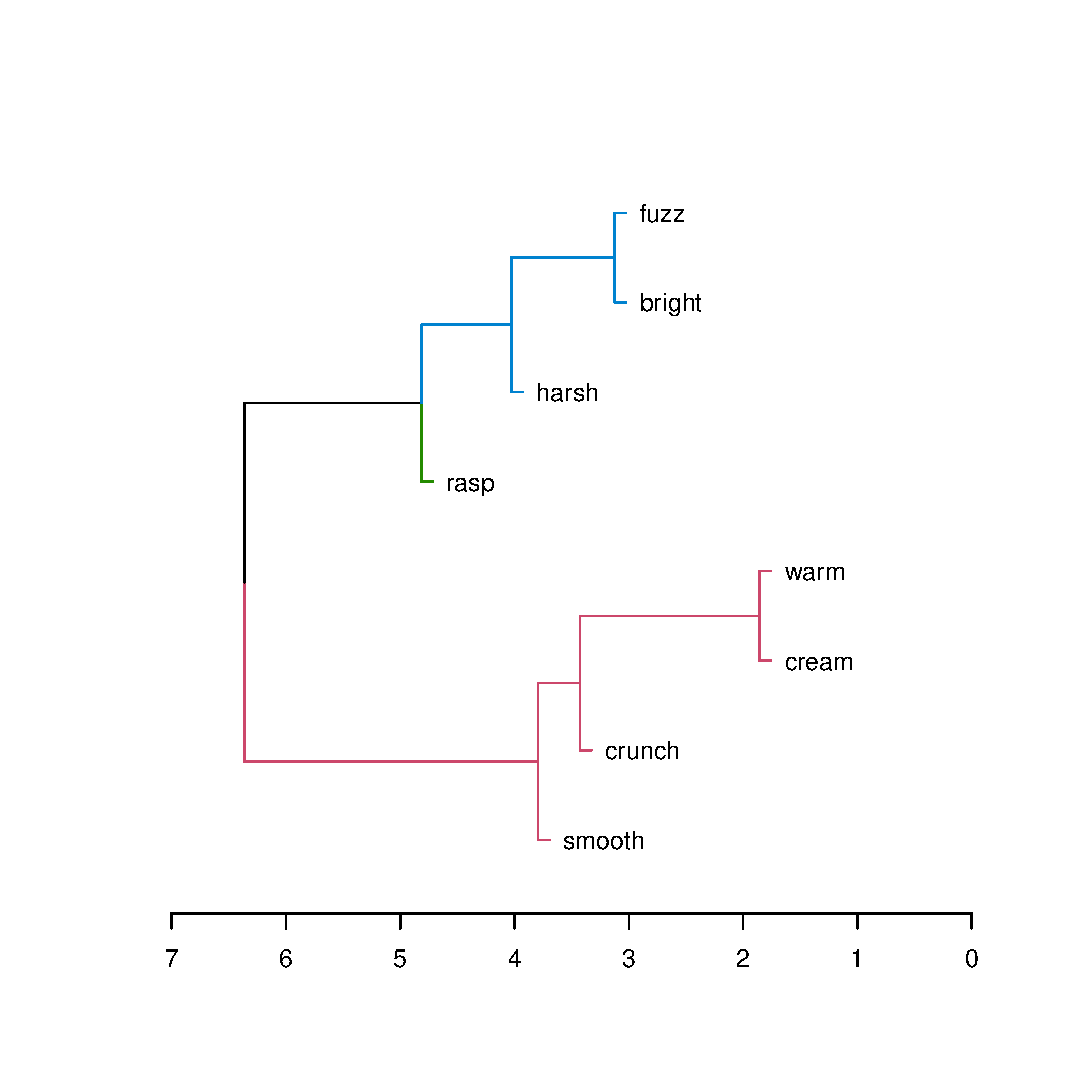
\includegraphics[width=0.45\textwidth]{chapter4/Images/DistortionDifferenceClusters.eps}
				\label{fig:DistortionDifferenceClusters}
			}
			\caption{Clustering of descriptors from the distortion.}
			\label{fig:DistortionClusters}
		\end{figure}
		
		The clusters identified in the equaliser (Figure \ref{fig:EqualiserClusters}) show less agreement between
		the two different feature spaces. While the terms `warm' and `bright' were the most distant from each other
		in the distortion feature spaces, they are two of the closest terms in the equaliser's processed feature
		space (Figure \ref{fig:EqualiserProcessedClusters}). They are, however, separated well in the equaliser's
		feature difference space (Figure \ref{fig:EqualiserDifferenceClusters}) suggesting that these terms better
		describe a certain change in audio features rather than an absolute feature value.

		\note
		{
			Probably due to the large number of instances of bright and warm. There is a wide range of input
			signals meaning the processed features average out to be similar. The underlying transforms are
			distinct for each descriptor however.
		}
		
		Within the equaliser's feature differences space two main clusters are identified corresponding with the
		`warmth' and `brightness' clusters from the distortion feature spaces. The `warmth' cluster includes the
		terms `deep' and `full' while the `brightness' cluster includes the terms `thin', `clear' and `air'. An
		additional `boominess' cluster, containing `mud', `boom' and `box', is also present. These three terms
		cluster better in the processed feature space indicating that they are more likely to describe a particular
		set of feature values rather than the properties of a transform.

		\begin{figure}[h!]
%		This figure is da baddest figure, ask your dyslexic down syndromed mother.
			\centering
			\subfloat[Processed Features]
			{
				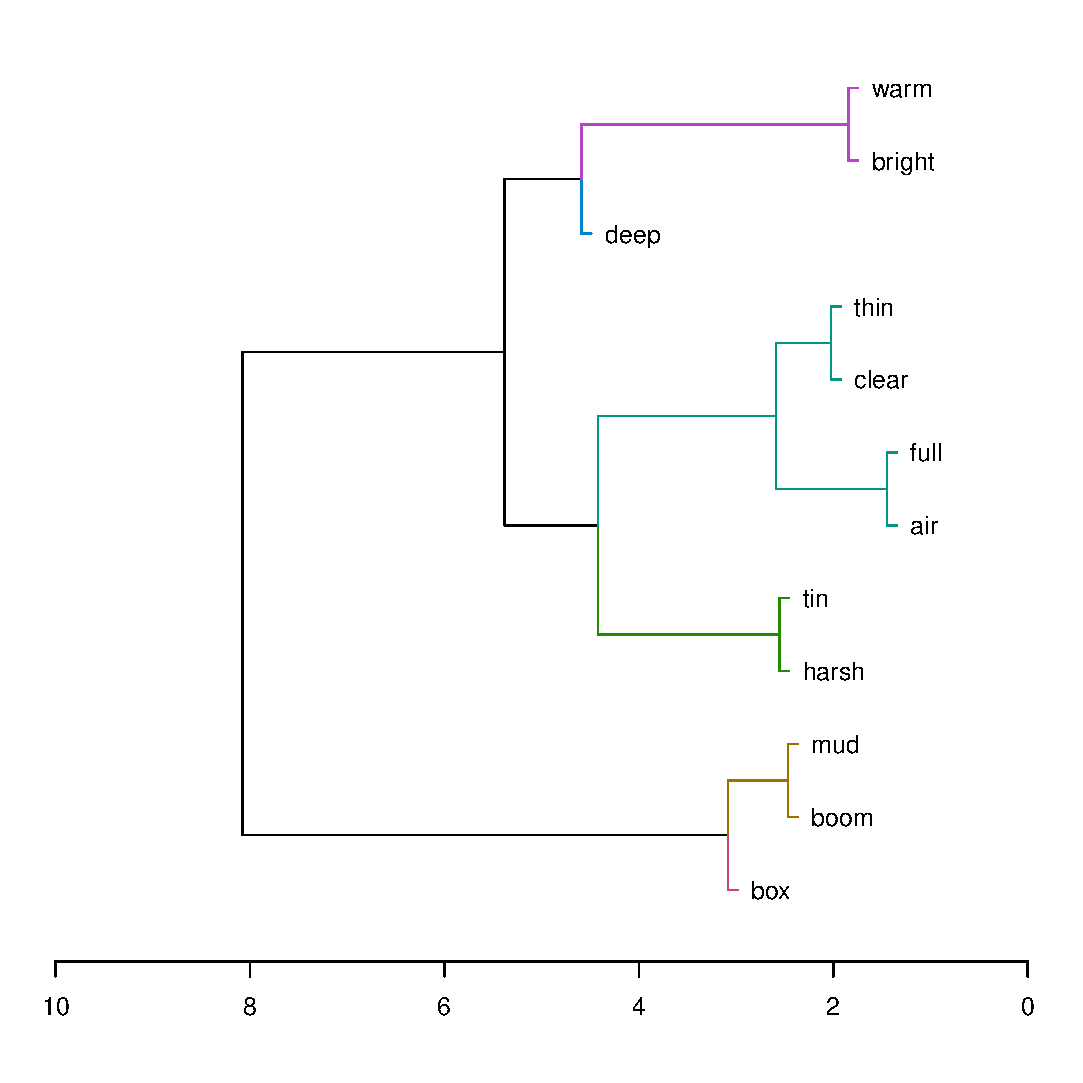
\includegraphics[width=0.45\textwidth]{chapter4/Images/EqualiserProcessedClusters.eps}
				\label{fig:EqualiserProcessedClusters}
			}
			\qquad
			\subfloat[Feature Differences]
			{
				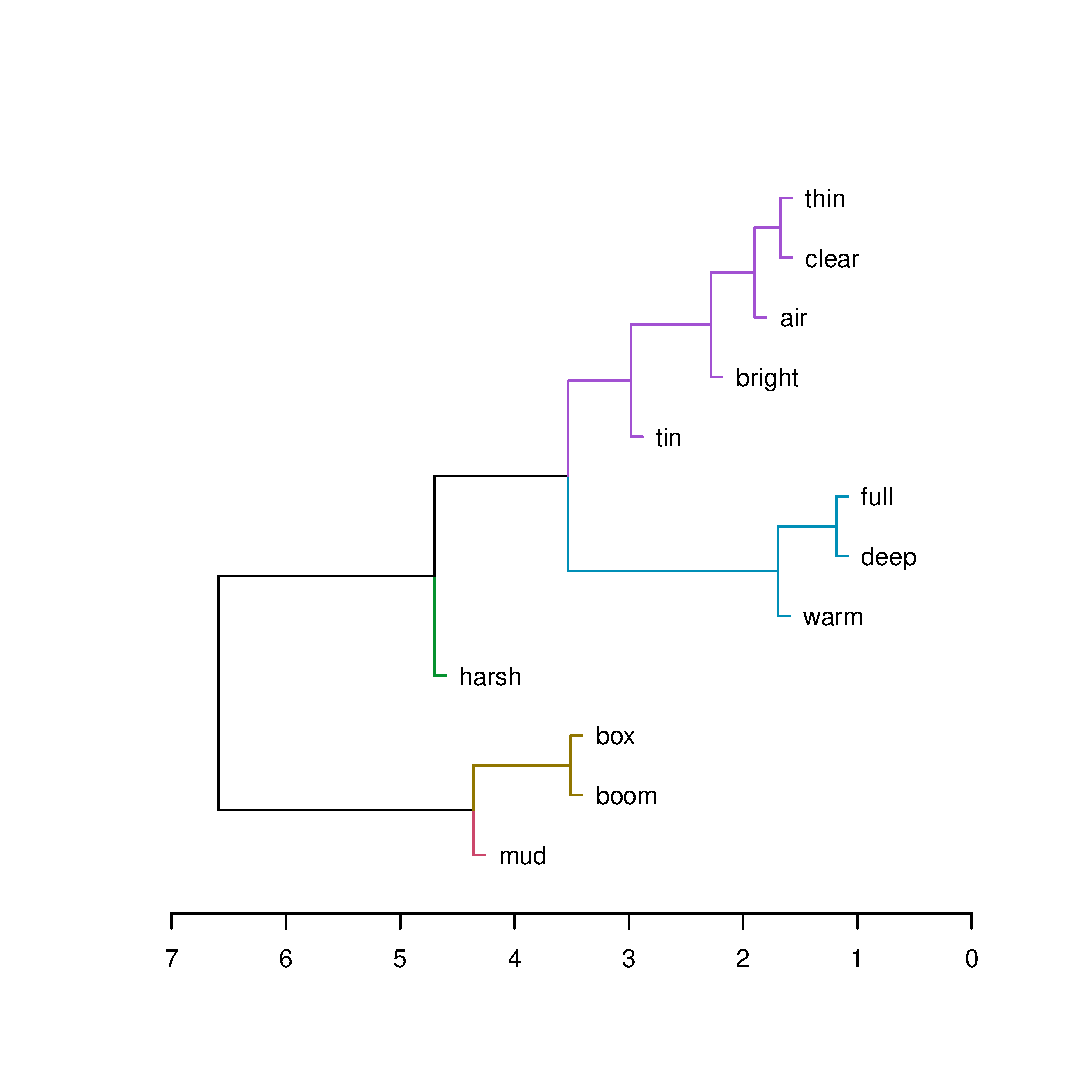
\includegraphics[width=0.45\textwidth]{chapter4/Images/EqualiserDifferenceClusters.eps}
				\label{fig:EqualiserDifferenceClusters}
			}
			\caption{Clustering of descriptors from the equaliser.}
			\label{fig:EqualiserClusters}
		\end{figure}
		
		In order to investigate the similarity of descriptors across both plug-ins their respective feature spaces
		are combined and clustering applied to produce the dendrograms shown in Figure \ref{fig:CombinedClusters}.
		Each descriptors is prepended with the name of the plug-in it is associated with.

		\begin{figure}[h!]
			\centering
			\subfloat[Processed Features]
			{
				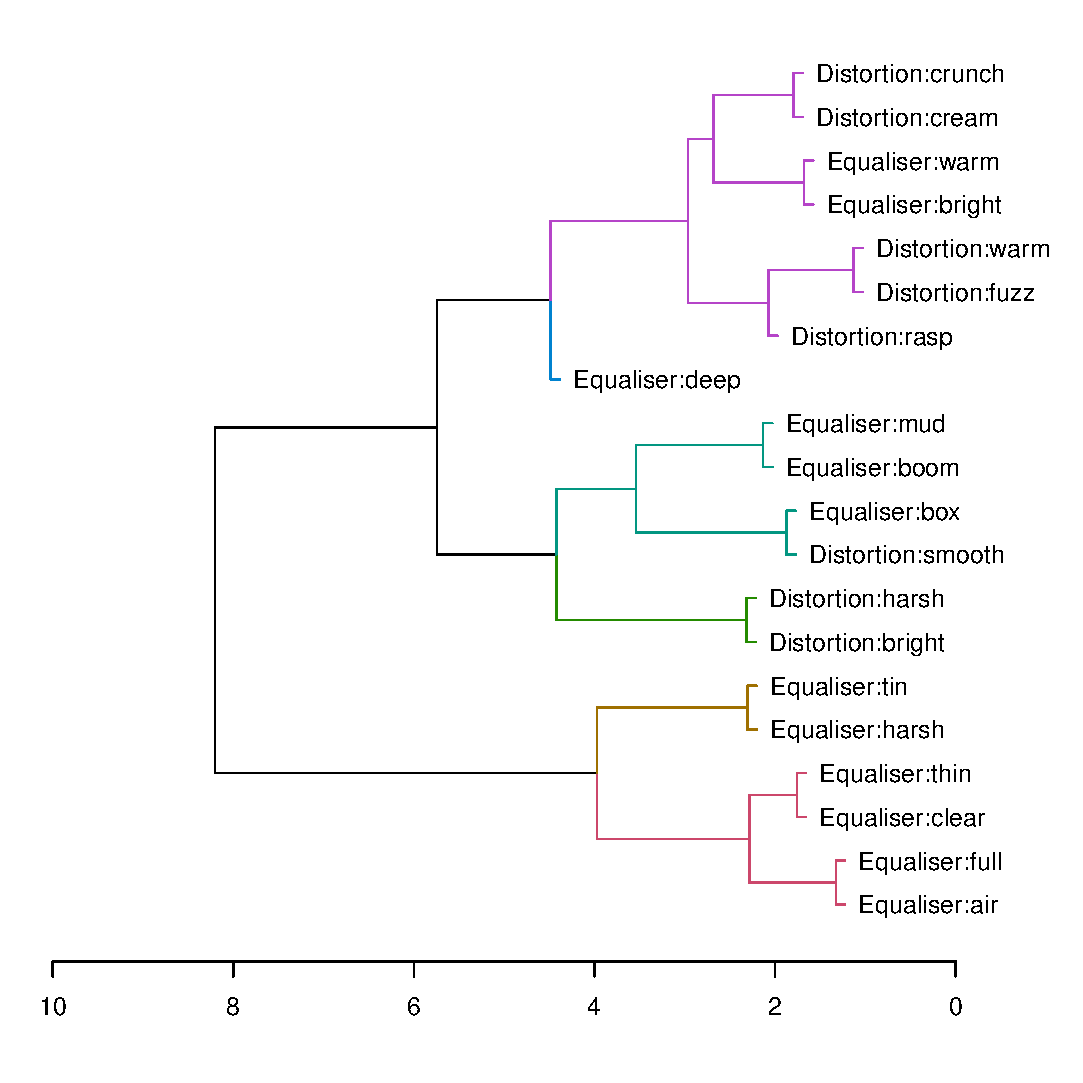
\includegraphics[width=0.45\textwidth]{chapter4/Images/CombinedProcessedClusters.eps}
				\label{fig:CombinedProcessedClusters}
			}
			\qquad
			\subfloat[Feature Differences]
			{
				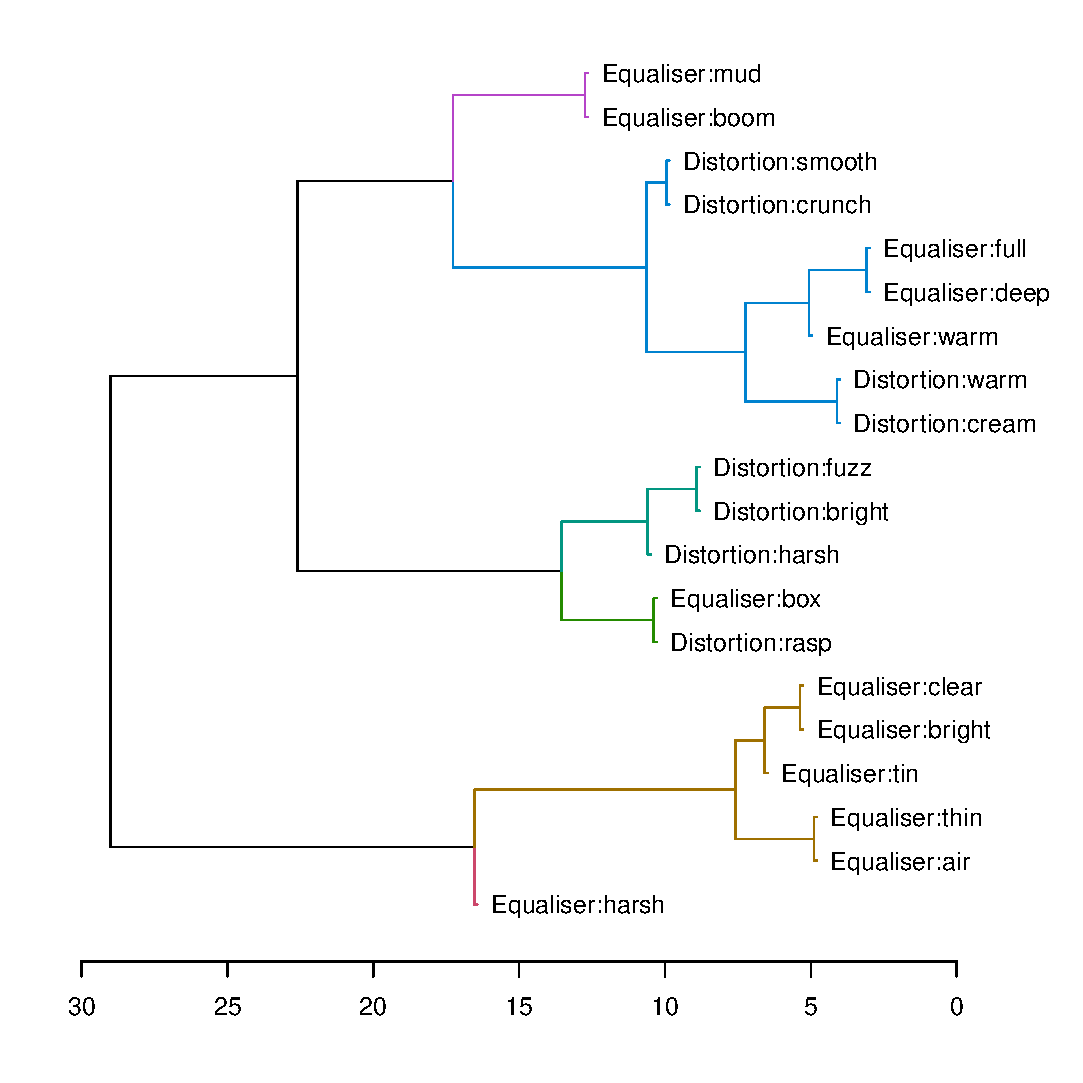
\includegraphics[width=0.45\textwidth]{chapter4/Images/CombinedDifferenceClusters.eps}
				\label{fig:CombinedDifferenceClusters}
			}
			\caption{Clustering of descriptors from the both the distortion and equaliser.}
			\label{fig:CombinedClusters}
		\end{figure}

		Here the `warmth' clusters from each plug-in's features spaces are combined, indicating that each of these
		descriptors describe similar transforms regardless of the processing method used. In contrast the
		`brightness' groups remain separated into clusters comprised mostly of descriptors from a single plug-in,
		suggesting that the use of these terms may differ depending on the nature of the audio transform.  Further
		evidence of this is found in the similarity of the terms `bright' and `harsh'. When used to describe
		distortion transforms these terms always sit adjacent to one another in a cluster, whereas for equaliser
		transforms they are separated by a reasonable distance. These terms are more likely to be synonymous when
		describing audio processed by a static nonlinearity then they are for equalised audio.

		The finer detail of the additional groups from the separate feature spaces (`crunchiness' and `boominess')
		are lost in the combined feature spaces. Each of these terms are clustered with terms from their associated
		plug-in, highlighting the timbral similarity between all signals processed by the same effect.

	\subsection{Agreement}
	\label{sec:TimbreEvaluation-Analysis-Agreement}
		In order to draw conclusions about the region a descriptor covers in a feature space, it is necessary to
		have a measure of agreement for a descriptor. This measure describes the level to which different users
		agree on the semantic meaning of descriptive terms. The closer together the transforms associated with a
		particular descriptor are grouped in the feature space, the higher that descriptor's agreement score.

		\citet{cartwright2013socialeq} measure how well participants agree on the semantic annotation of graphic
		equaliser parameter settings. For each participant a set of weightings is produced which describes the
		influence of each equaliser band on the perception of a particular timbral descriptor. The agreement score
		for a descriptor, $A(d)$, measures how similar these weightings are across different test participants
		using Equation \ref{eq:SocialEqAgreement}.

		\begin{equation}
			A(d) = \frac{\ln(N_{d})}{\sum_{k = 1}^{K} s_{d,k}^{2}}
			\label{eq:SocialEqAgreement}
		\end{equation}

		Where $N_{d}$ is the number of participants which have provided weightings for descriptor $d$,
		$s_{d,k}^{2}$ is the variance of weighting $k$ across those participants and $K$ is the number of
		weightings in each set (i.e. the number of equaliser bands). The logarithm of the number of
		participants is used to account for Zipf's law, which states that the frequency with which a word is used
		is inversely proportional to its usage ranking (an integer describing the words popularity; 1 denoting the
		most commonly used word, 2 the second most common etc.) \citep{manning1999foundations}.

		This can be applied to data from the SAFE plug-ins by using audio feature values in place of parameter
		weightings. In Equation \ref{eq:SocialEqAgreement}, $N_{d}$ is then the number of transforms labelled with
		descriptor $d$, $s_{d,k}^{2}$ is the variance of feature $k$ across those transforms and $K$ is the
		number of features. As when clustering, the feature space should be standardised prior to calculating
		agreement to remove the biasing effects caused by the ranges of each feature.

		This agreement measure has several properties which do not necessarily reflect what is being measured:

		\begin{itemize}
			\item A larger number of transforms, $N_{d}$, produces higher agreement.
			\item It is assumed that high variance in any feature implies a disagreement. 
			\item It is assumed that all audio features are independent. 
			\item It is assumed that low variance in any feature implies an agreement. 
		\end{itemize}

		In this section an agreement measure which accounts for these points is developed.

		\subsubsection*{Number of Transforms}
			In Equation \ref{eq:SocialEqAgreement} the logarithm of the number of transforms, $N_{d}$, is used
			to scale the agreement score. This measures a different concept of agreement to what we desire for
			this work. Rather than measuring the size of the region a descriptor occupies in the feature space,
			it measure how many individual transforms make up that region. A sufficiently large number of
			transforms will produce a large agreement score regardless of how spread apart they are. To measure
			the size of the region a descriptor occupies, the scaling factor should be removed giving Equation
			\ref{eq:ReciprocalOfSumAgreement}.

			\begin{equation}
				A(d) = \frac{1}{\sum_{k = 1}^{K} s_{d,k}^{2}}
				\label{eq:ReciprocalOfSumAgreement}
			\end{equation}

			To take account of the number of transforms labelled with a particular descriptor, Bessel's
			correction can be used in the calculation of variance as shown in Equation
			\ref{eq:UnbiasedVariance}. This uses the data available from a sample and uses it to approximate
			the variation present in the population.

			\begin{equation}
				s_{d,k}^{2} = \frac{1}{N_{d} - 1} \sum_{n = 1}^{N_{d}} (x_{d,k,n} - \bar{x}_{d,k})^{2}
				\label{eq:UnbiasedVariance}
			\end{equation}

			Where $x_{d,k,n}$ is the value of feature $k$ for the $n$\super{th} transform labelled with
			descriptor $d$ and $\bar{x}_{d,k}$ is the mean value of feature $k$ across all transforms labelled
			with descriptor $d$.

			Using this measure of variance in the agreement score provides an approximation of how closely
			clustered transforms, labeled with a certain descriptor, would be in a feature space which
			represents the whole population. In all further agreement score calculations it is assumed that the
			variances, or covariances, are measured using Bessel's correction.

		\subsubsection*{High Variance}
			A term exhibiting high variance in a particular audio feature could imply one of two things. Either
			that users do not agree on the position of the term in the feature space, or that that feature has
			no effect on the perception of the term. In the first case the agreement score should be decreased,
			but in the second the agreement score should not be affected. Because of this ambiguity, it is
			preferable that a high variance has negligible effect on the agreement score. In this way, if a
			high variance does imply disagreement it does not unduly increase the agreement score and if at
			does not imply disagreement it does to unduly decrease the agreement score.
			
			This can be implemented by changing Equation \ref{eq:ReciprocalOfSumAgreement} to be a sum of
			reciprocals rather than the reciprocal of a sum, as shown in Equation
			\ref{eq:SumOfReciprocalAgreement}.

			\begin{equation}
				A(d) = \sum_{k = 1}^{K} \frac{1}{s_{d,k}^{2}}
				\label{eq:SumOfReciprocalAgreement}
			\end{equation}

		\subsubsection*{Dependent Features}
			It may be the case that users agree that a particular term describes a relationship between several
			audio features (e.g. a spectral centroid lying at the 4\super{th} harmonic). Equations
			\ref{eq:SocialEqAgreement}, \ref{eq:ReciprocalOfSumAgreement} and \ref{eq:SumOfReciprocalAgreement}
			all ignore any dependence between audio features.

			Relationships between features can be taken into account by calculating the covariance matrix for
			the transforms associated with a term. The variances in each feature can then be substituted with
			the eigenvalues of this matrix, as shown in Equation \ref{eq:EigenvalueAgreement}.

			\begin{equation}
				A(d) = \sum_{k = 1}^{K} \frac{1}{\lambda_{d,k}}
				\label{eq:EigenvalueAgreement}
			\end{equation}
			
			Where $\lambda_{d, k}$ is the $k$\super{th} eigenvalue of the covariance matrix for all transforms
			labelled with descriptor $d$.

			When using Equation \ref{eq:EigenvalueAgreement}, the number of eigenvalues used, $K$, needs to be
			carefully selected. If $N_{d}$ is less than or equal to the total number of audio features the
			covariance matrix will be singular, meaning it will have one or more eigenvalues equal to zero. At
			most, only the $N_{d} - 1$ largest eigenvalues should be used in order to avoid the agreement score
			becoming undefined.

			Any other zero eigenvalues would imply a perfect linear relationship between a combination of audio
			features. \note{Can I just say we will ignore that for now? It is a very unlikely occurrence,
			disregarding features which are defined to be linearly related (which will get fixed by PCA).}

		\subsubsection*{Validation with Synthesised Data}
			To demonstrate the differences between Equations \ref{eq:SocialEqAgreement},
			\ref{eq:SumOfReciprocalAgreement} and \ref{eq:EigenvalueAgreement} artificial data can be
			synthesised which exhibits some of the issues discussed with Equation \ref{eq:SocialEqAgreement}.
			
			\note
			{
				Data synthesised as done by \citet{ripley1987stochastic}.
			}

			Figure \ref{fig:SynthesisedData} show a synthesised, three dimensional, dataset containing four
			clusters of points. Each cluster has different properties which need to be taken into account when
			calculating the agreement score. Cluster 1 represents a set of points whose position in the feature
			space is not agreed upon, exhibiting a high variance in every feature. Cluster 2 represents a set
			of points whose position is very well agreed upon, having low variance in every feature. Cluster 3
			represents a set of points whose position is only defined in one audio feature, having high
			variance in the other two. Cluster 4 represent a set of points which are defined by a relationship
			between two features, exhibiting high variance in all features but a strong correlation ($p = 0.9$)
			between features 1 and 2.

			\note
			{
				How much detail should be given as to the generation of this data. Do we need to explicitly
				state each cluster covariances matrix? Do we need to mention the method used to generate
				the distributions? Reference the R documentation for mvrnorm perhaps, or name drop the
				algorithm that uses (which I don't know at the moment, come on inter library loan).
			}

			\begin{figure}[h!]
				\centering
				\subfloat
				{
					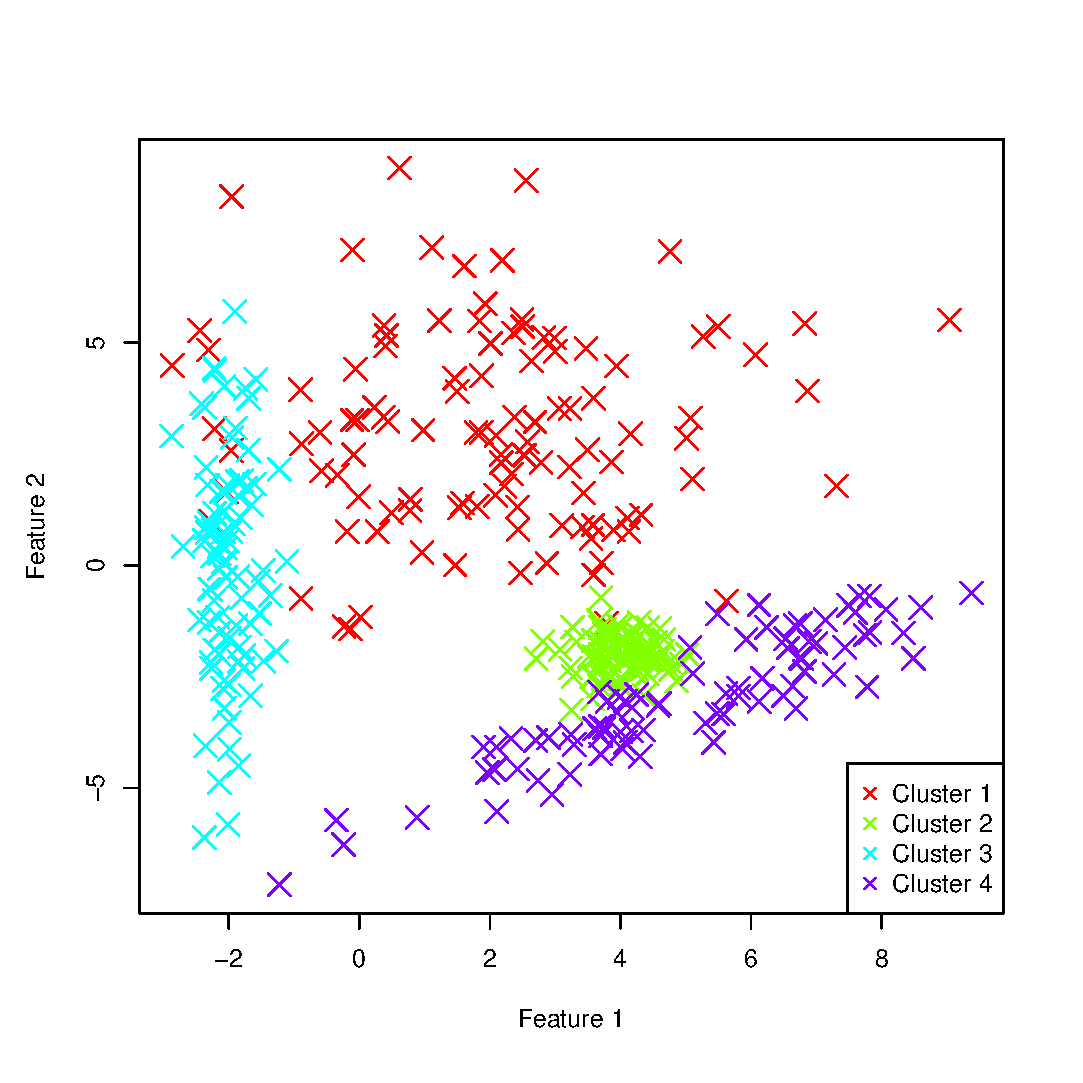
\includegraphics[width=0.45\textwidth]{chapter4/Images/ArtificialData1-2.eps}
					\label{fig:EqualiserDifferencePCA}
				}
				\qquad
				\subfloat
				{
					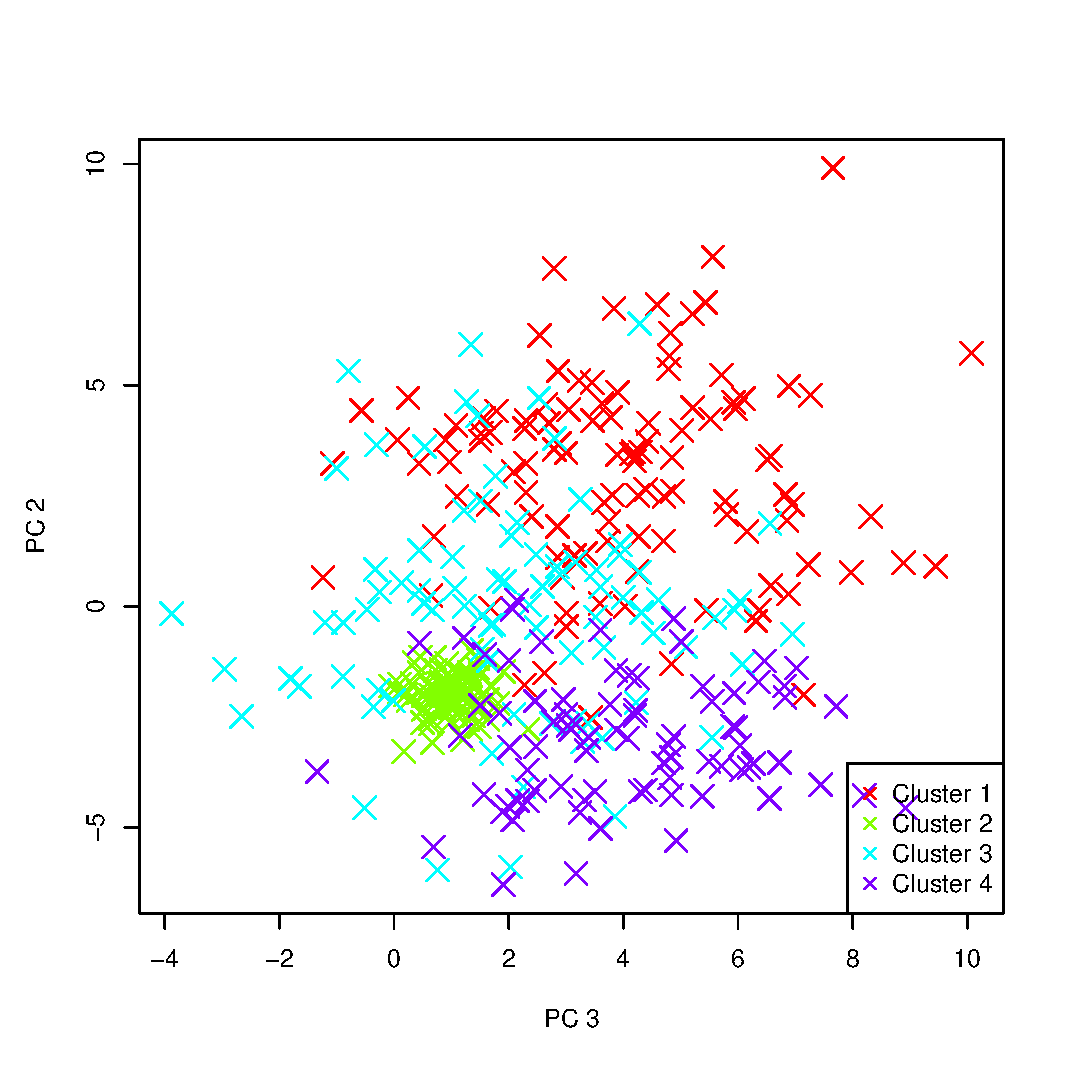
\includegraphics[width=0.45\textwidth]{chapter4/Images/ArtificialData3-2.eps}
					\label{fig:EqualiserDifferenceCentroidsPCA}
				}
				\caption{Synthesised Data}
				\label{fig:SynthesisedData}
			\end{figure}

			Visualising the data in Figure \ref{fig:SynthesisedData} provides intuition as to how an agreement
			score should rate each cluster. Cluster 1 should receive the lowest score as there is no
			discernible pattern to the data points. Cluster 2 should receive the highest score as it is very
			tightly clustered in all features. Both clusters 3 and 4 show some some patterns in the
			distribution. Cluster 3 has a well defined position in feature 1 while cluster 4 shows a strong
			relationship between features 1 and 2. The agreement scores for these clusters should reflect these
			patterns.

			Table \ref{tab:SynthesisedDataAgreement} shows agreement scores, for the data shown in Figure
			\ref{fig:SynthesisedData}, calculated using Equations \ref{eq:SocialEqAgreement},
			\ref{eq:SumOfReciprocalAgreement} and \ref{eq:EigenvalueAgreement}.

			\begin{table}[h!]
				\centering
				\begin{tabular}{|c|c|c|c|c|}
					\cline{2-5}
					\multicolumn{1}{c|}{} & \multicolumn{4}{c|}{\bf{Agreement Score}} \tabularnewline
					\hline
					\bf{Cluster} & \bf{Equation \ref{eq:SocialEqAgreement}} & 
					\bf{Equation \ref{eq:ReciprocalOfSumAgreement}} &
					\bf{Equation \ref{eq:SumOfReciprocalAgreement}} & 
					\bf{Equation \ref{eq:EigenvalueAgreement}} \tabularnewline
					\hline
					\hline
					\bf{1} & 2.3 & 0.5 & 4.7 & 4.7 \tabularnewline
					\hline
					\bf{2} & 55.1 & 12.2 & 117.9 & 117.9 \tabularnewline
					\hline
					\bf{3} & 2.7 & 0.6 & 95.7 & 95.7 \tabularnewline
					\hline
					\bf{4} & 2.9 & 0.7 & 7.7 & 34.8 \tabularnewline
					\hline
				\end{tabular}
				\caption{Agreement Scores for Synthesised Data}
				\label{tab:SynthesisedDataAgreement}
			\end{table}

			The issues with Equation \ref{eq:SocialEqAgreement} are immediately obvious, it ignores readily
			noticeable patterns in the data giving clusters 1, 3 and 4 similar agreement scores. By removing
			the assumption that high variance implies disagreement, Equation \ref{eq:SumOfReciprocalAgreement}
			takes account of the pattern in cluster 3. Equation \ref{eq:EigenvalueAgreement} remove the
			assumption that all features are independent enabling it to reflect the pattern shown in cluster 4.

			\note
			{
				I am also concerned about how unbounded these values are. I was thinking of using $1 +
				s_{d,k}^{2}$ to bound it.
			}

		\subsubsection*{Low Variance}
			Low variance in a particular audio feature does not necessarily imply an agreement between users.
			It may indicate a similarity between all of the audio segments processed, regardless of semantic
			labelling. To account for this features which have low variance across the entire dataset can be
			disregarded. This can be achieved by calculating the agreement in a reduced dimensionality feature
			space.

			Using PCA the dimensions with the largest variance in the feature space can be discovered. If the
			transforms labelled with a particular term exhibit a small variance in one of these dimensions it
			is likely that that term is well agreed upon. Agreement can be calculated in the PCA timbre space
			using Equation \ref{eq:EigenvalueAgreement} with $\lambda_{d,k}$ being the $k$\super{th} eigenvalue
			of the covariance matrix for every transform labelled with descriptor $d$ in the first $K$
			principal components. As when calculating the agreement in the feature space, the coordinates of
			the transforms in each principal component should be standardised to remove bias introduced by the
			proportions of total variance each component describes.

			The number of principal components to use in the calculation of agreement will depend on the
			dataset being analysed. Two considerations help in the selection of this number. Firstly, only
			principal components with eigenvalues greater than a certain value should be retained. Only in
			these components can a low variance be interpreted as agreement between users. Secondly the number
			of transforms labelled with a each descriptor should be taken into account. Using a number of
			principal components which is less than the size of the smallest group of transforms avoids the
			occurrence of zero valued eigenvalues caused by insufficient data points.

	\subsection{Timbre Spaces}
	\label{sec:TimbreEvaluation-Analysis-TimbreSpaces}
		Clustering provides insight into the similarity of descriptive terms but does not show what properties of
		the signals / transforms contribute to the differences between descriptor clusters. Reducing the
		dimensionality of the audio feature space allows for the most salient features to be identified. To
		preserve as much of the audio feature data as possible, a different feature space, to that used for
		clustering, is constructed. Rather than each descriptor representing one point in the feature space, each
		individual transform, labeled with a certain descriptor, represents its own point. In this manner
		dimensions which have little effect on a certain timbral descriptor are easily determined. The points
		labeled with a particular term will be more spread out across the dimensions which do not affect them. 
		
		Prior to analysis, the feature spaces are standardised to remove any bias caused by features with a large
		range. PCA is then applied in order to create the low dimensionality timbre spaces discussed in this
		section. Salient audio features are identified through taking correlation measures between the original
		audio feature values and the coordinates of terms in the timbre space.

		\note
		{
			Do we really need both of the plots for each space. If so probably put a paragraph here explaining
			the difference between the two.
		}

		\begin{figure}[h!]
			\centering
			\subfloat[Individual Transforms]
			{
				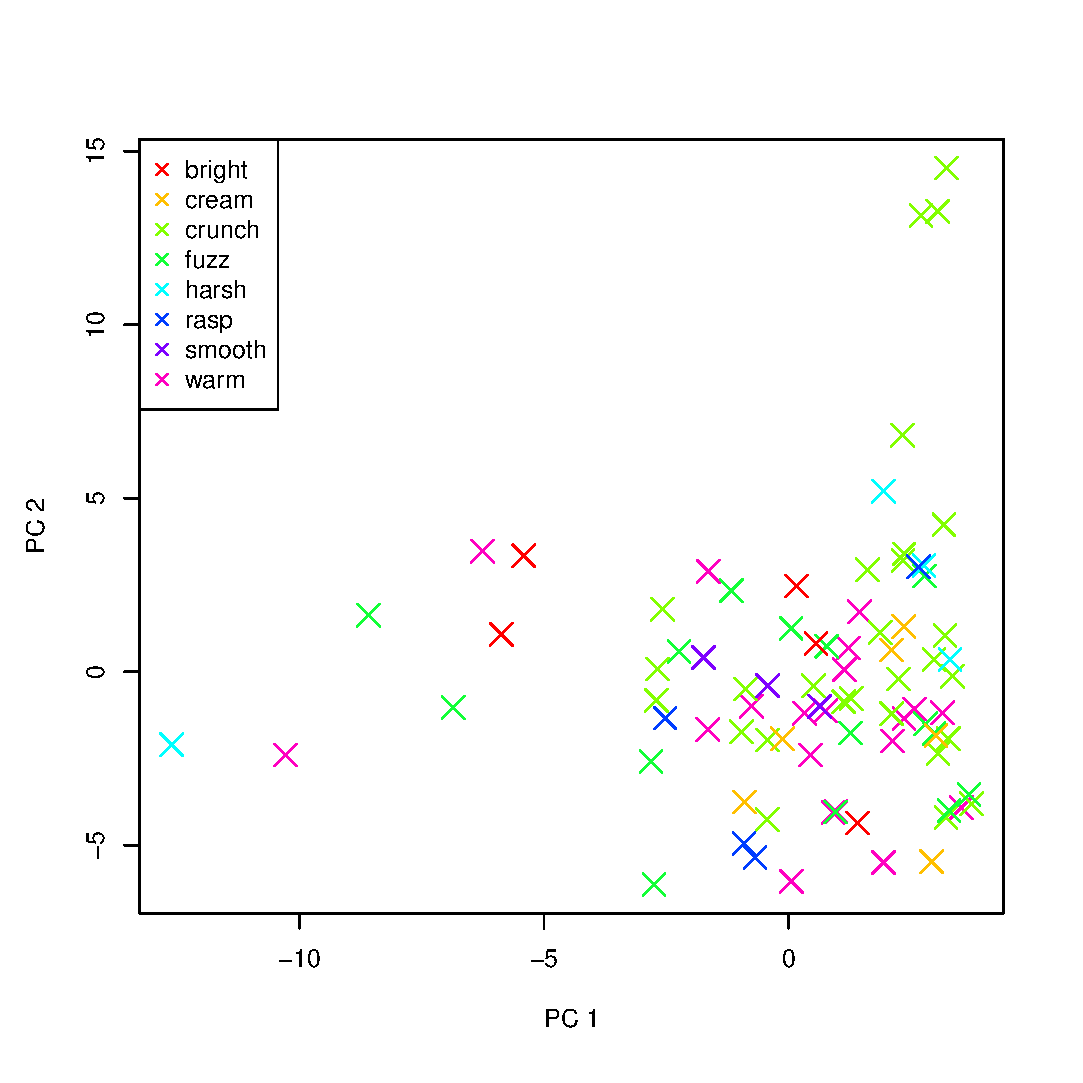
\includegraphics[width=0.45\textwidth]{chapter4/Images/DistortionProcessedPCA.eps}
				\label{fig:DistortionProcessedPCA}
			}
			\qquad
			\subfloat[Descriptor Centroids]
			{
				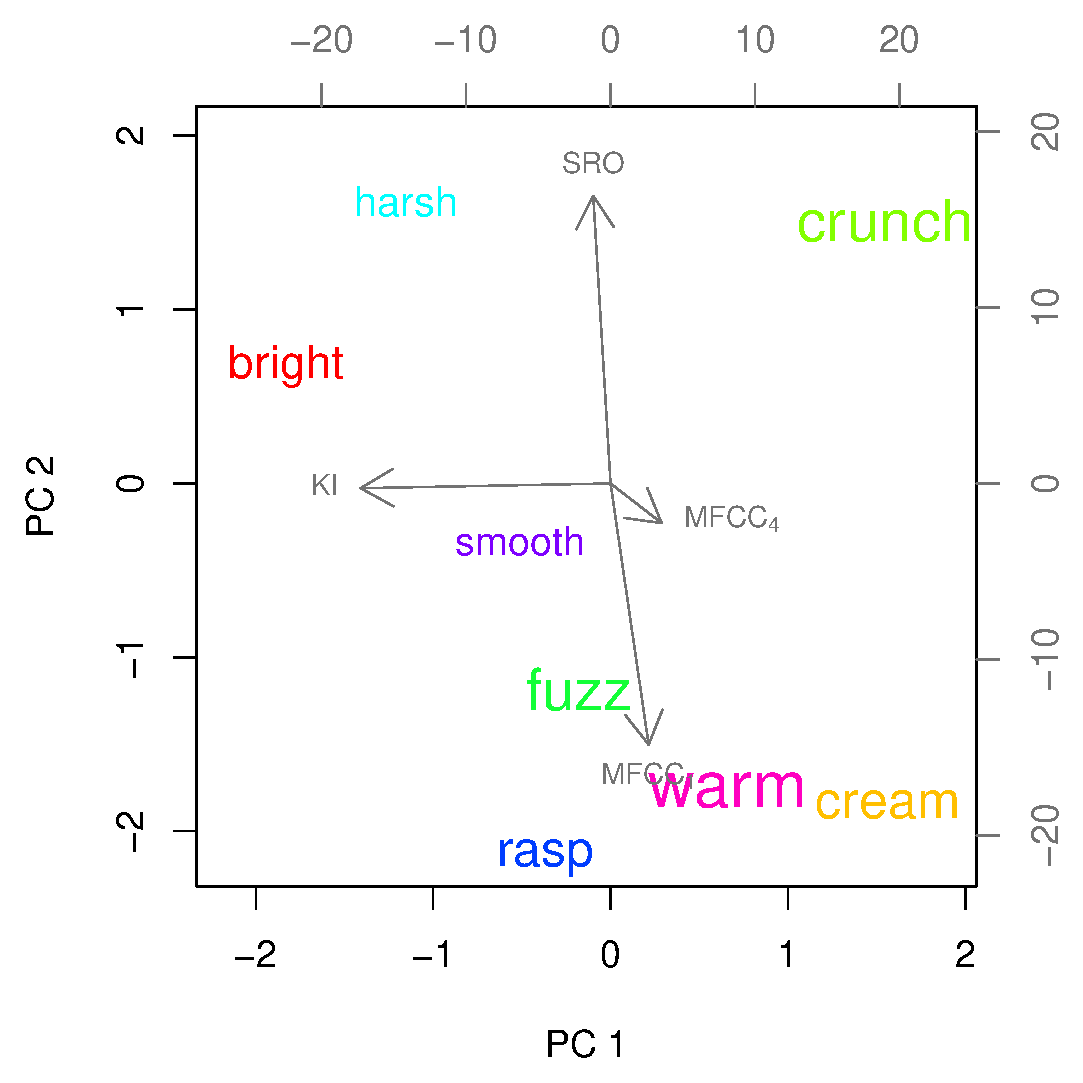
\includegraphics[width=0.45\textwidth]{chapter4/Images/DistortionProcessedCentroidsPCA.eps}
				\label{fig:DistortionProcessedCentroidsPCA}
			}
			\caption{Timbre space for the processed features from the distortion.}
			\label{fig:DistortionProcessedPCAs}
		\end{figure}

		\begin{table}[h!]
			\centering
			\begin{tabular}{|c|c|c|c|c|c|}
				\cline{2-6}
				\multicolumn{1}{c|}{} & \multicolumn{5}{c|}{\bf{Correlation}} \tabularnewline
				\hline
				\bf{Feature} & \bf{PC1} & \bf{PC2} & \bf{PC3} & \bf{PC4} & \bf{PC5} \tabularnewline
				\hline
				\hline
				\bf{Krimphoff Irregularity} & \bf{-0.984} & -0.0238 & -0.0969 & 0.0537 & -0.0265 \tabularnewline
				\hline
				\bf{Peak Krimphoff Irregularity} & \bf{-0.971} & 0.0529 & -0.102 & 0.122 & 0.0252 \tabularnewline
				\hline
				\bf{Peak Spectral Kurtosis} & \bf{-0.952} & 0.021 & -0.136 & 0.126 & -0.123 \tabularnewline
				\hline
				\bf{Peak Spectral Skewness} & \bf{-0.94} & 0.105 & -0.14 & 0.168 & -0.0884 \tabularnewline
				\hline
				\bf{Harmonic Krimphoff Irregularity} & \bf{-0.937} & 0.145 & -0.114 & 0.214 & 0.0292 \tabularnewline
				\hline
				\bf{Harmonic Spectral Kurtosis} & \bf{-0.937} & 0.0868 & -0.139 & 0.201 & -0.0787 \tabularnewline
				\hline
				\bf{Spectral Roll Off} & 0.114 & \bf{-0.929} & -0.1 & 0.143 & 0.174 \tabularnewline
				\hline
				\bf{Spectral Skewness} & \bf{-0.924} & 0.168 & 0.00408 & 0.214 & 0.142 \tabularnewline
				\hline
				\bf{Spectral Centroid} & 0.089 & \bf{-0.922} & -0.273 & 0.0801 & -0.00138 \tabularnewline
				\hline
				\bf{Harmonic Spectral Skewness} & \bf{-0.922} & 0.17 & -0.155 & 0.221 & -0.0305 \tabularnewline
				\hline
				\bf{Spectral Slope} & 0.127 & \bf{-0.893} & -0.228 & 0.132 & -0.0603 \tabularnewline
				\hline
				\bf{Peak Spectral Standard Deviation} & 0.162 & \bf{-0.891} & -0.0698 & 0.277 & 0.234 \tabularnewline
				\hline
				\bf{Harmonic Spectral Standard Deviation} & 0.172 & \bf{-0.891} & -0.0804 & 0.281 & 0.236 \tabularnewline
				\hline
				\bf{Harmonic Spectral Centroid} & 0.199 & \bf{-0.87} & -0.0738 & 0.312 & 0.251 \tabularnewline
				\hline
				\bf{Peak Spectral Centroid} & 0.198 & \bf{-0.869} & -0.0711 & 0.31 & 0.259 \tabularnewline
				\hline
				\bf{MFCC 1} & 0.0573 & \bf{0.869} & -0.1 & 0.242 & -0.094 \tabularnewline
				\hline
				\bf{Signal Standard Deviation} & \bf{-0.854} & 0.256 & -0.291 & 0.243 & 0.035 \tabularnewline
				\hline
				\bf{RMS Amplitude} & \bf{-0.854} & 0.256 & -0.291 & 0.243 & 0.0346 \tabularnewline
				\hline
				\bf{MFCC 4} & 0.135 & -0.116 & \bf{-0.82} & -0.114 & -0.169 \tabularnewline
				\hline
				\bf{Zero Crossing Rate} & 0.145 & \bf{-0.817} & -0.0682 & 0.111 & 0.283 \tabularnewline
				\hline
			\end{tabular}
			\caption{Correlations between audio features and principal components for Figure
				 \ref{fig:DistortionProcessedPCAs}}
			\label{fig:DistortionProcessedCorrelations}
		\end{table}

		\begin{figure}[h!]
			\centering
			\subfloat[Individual Transforms]
			{
				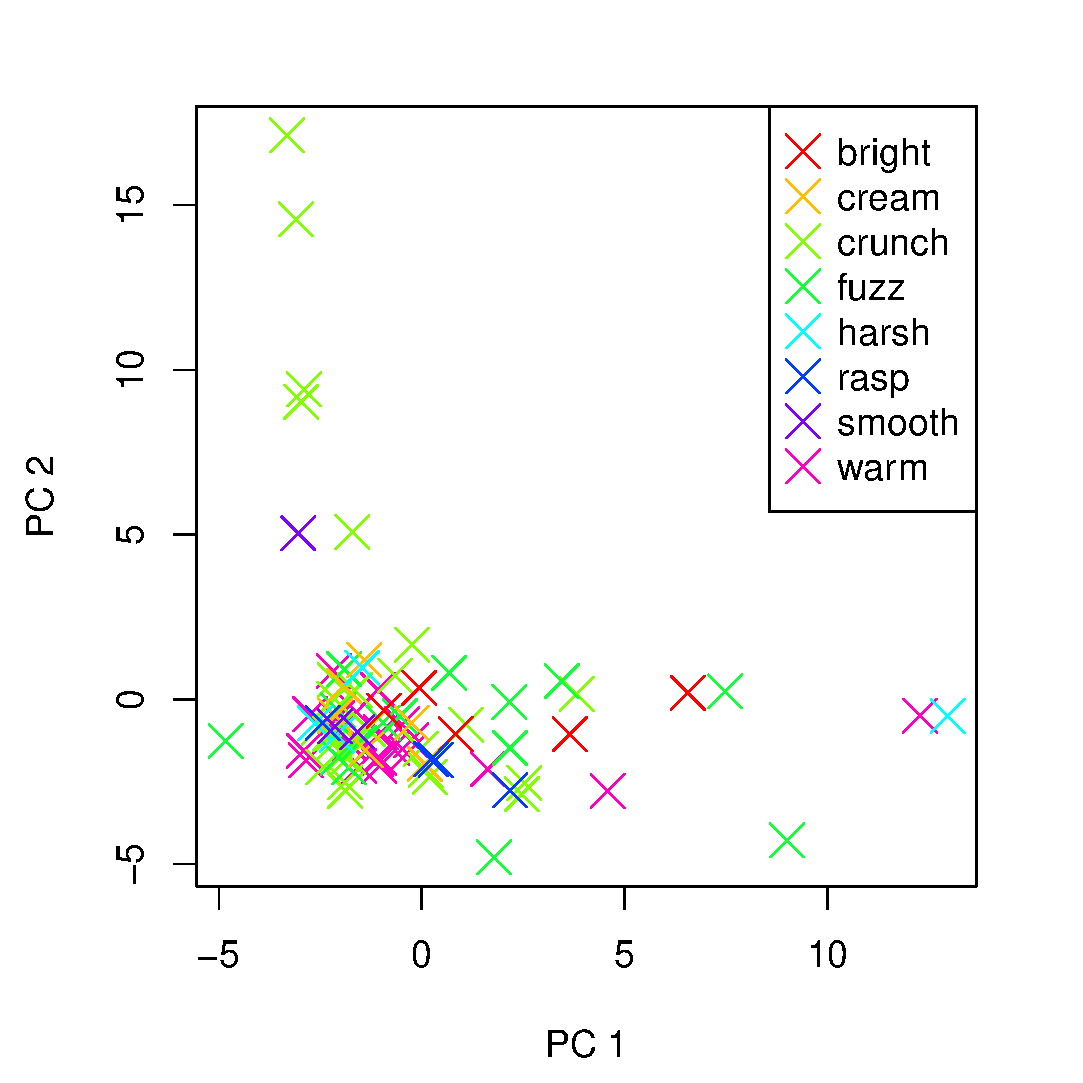
\includegraphics[width=0.45\textwidth]{chapter4/Images/DistortionDifferencePCA.eps}
				\label{fig:DistortionDifferencePCA}
			}
			\qquad
			\subfloat[Descriptor Centroids]
			{
				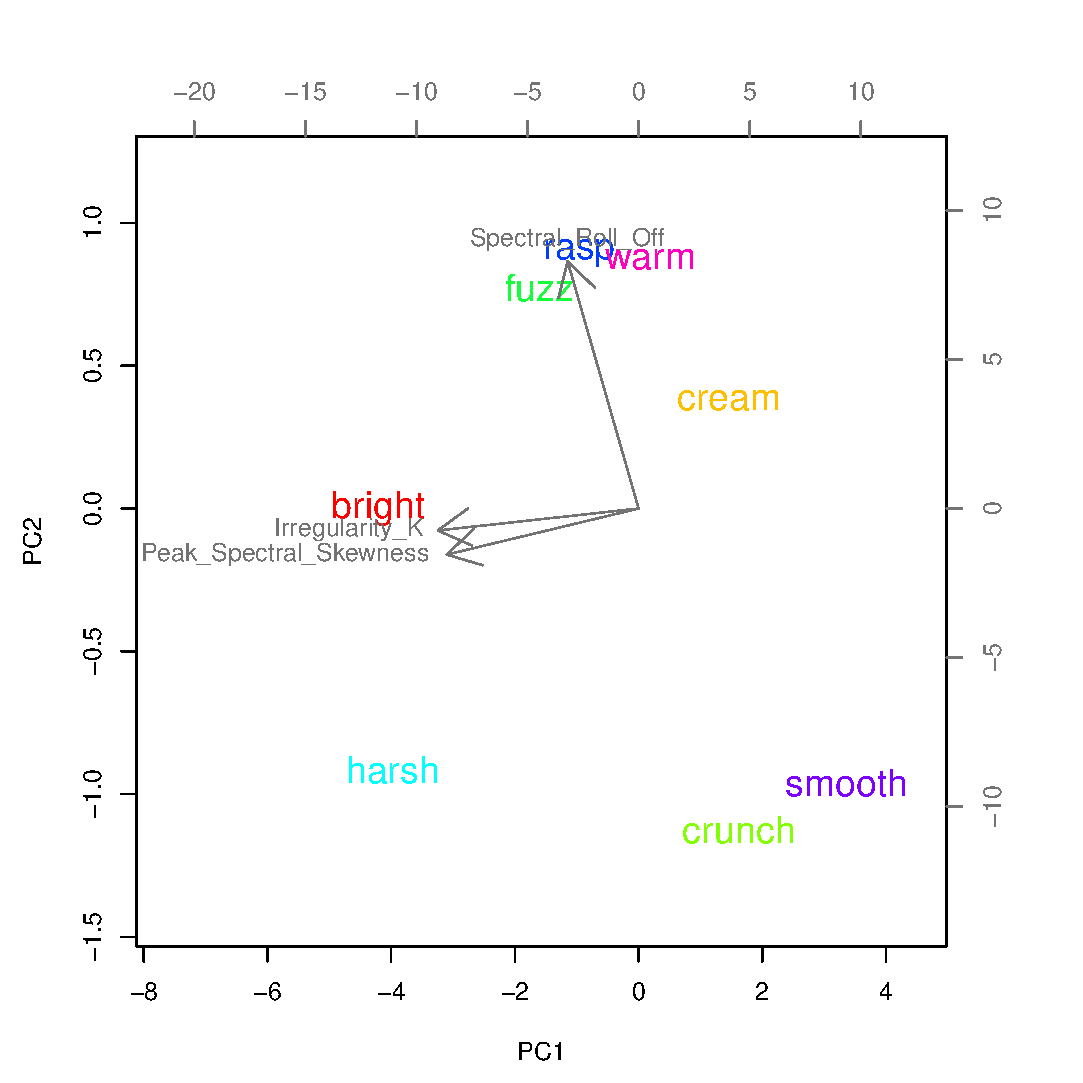
\includegraphics[width=0.45\textwidth]{chapter4/Images/DistortionDifferenceCentroidsPCA.eps}
				\label{fig:DistortionDifferenceCentroidsPCA}
			}
			\caption{Timbre space for the feature differences from the distortion.}
			\label{fig:DistortionDifferencePCAs}
		\end{figure}

		\begin{table}[h!]
			\centering
			\begin{tabular}{|c|c|c|c|c|c|}
				\cline{2-6}
				\multicolumn{1}{c|}{} & \multicolumn{5}{c|}{\bf{Correlation}} \tabularnewline
				\hline
				\bf{Feature} & \bf{PC1} & \bf{PC2} & \bf{PC3} & \bf{PC4} & \bf{PC5} \tabularnewline
				\hline
				\hline
				\bf{Krimphoff Irregularity} & \bf{-0.986} & -0.0805 & 0.0147 & -0.0516 & -0.0494 \tabularnewline
				\hline
				\bf{Peak Krimphoff Irregularity} & \bf{-0.978} & -0.107 & 0.0833 & 0.0504 & 0.0287 \tabularnewline
				\hline
				\bf{Harmonic Krimphoff Irregularity} & \bf{-0.959} & -0.106 & 0.2 & 0.0252 & 0.0557 \tabularnewline
				\hline
				\bf{Peak Spectral Skewness} & \bf{-0.942} & -0.169 & 0.182 & 0.119 & 0.0132 \tabularnewline
				\hline
				\bf{Harmonic Spectral Skewness} & \bf{-0.93} & -0.169 & 0.231 & 0.103 & 0.0497 \tabularnewline
				\hline
				\bf{Peak Spectral Kurtosis} & \bf{-0.927} & -0.178 & 0.163 & 0.156 & -0.045 \tabularnewline
				\hline
				\bf{Harmonic Spectral Kurtosis} & \bf{-0.912} & -0.18 & 0.236 & 0.153 & 0.00977 \tabularnewline
				\hline
				\bf{RMS Amplitude} & \bf{-0.907} & -0.157 & 0.197 & 0.22 & 0.107 \tabularnewline
				\hline
				\bf{Signal Standard Deviation} & \bf{-0.907} & -0.157 & 0.197 & 0.22 & 0.107 \tabularnewline
				\hline
				\bf{Spectral Roll Off} & -0.349 & \bf{0.905} & 0.147 & 0.064 & -0.0101 \tabularnewline
				\hline
				\bf{Spectral Spread} & -0.249 & \bf{0.893} & 0.0082 & 0.0152 & 0.145 \tabularnewline
				\hline
				\bf{Spectral Skewness} & \bf{-0.89} & -0.156 & 0.253 & 0.114 & 0.283 \tabularnewline
				\hline
				\bf{Harmonic Spectral Centroid} & -0.224 & \bf{0.886} & 0.172 & 0.258 & -0.035 \tabularnewline
				\hline
				\bf{Harmonic Spectral Standard Deviation} & -0.246 & \bf{0.879} & 0.178 & 0.203 & -0.0585 \tabularnewline
				\hline
				\bf{Peak Spectral Centroid} & -0.225 & \bf{0.87} & 0.157 & 0.262 & -0.0306 \tabularnewline
				\hline
				\bf{Spectral Centroid} & -0.393 & \bf{0.866} & -0.0119 & -0.15 & 0.0507 \tabularnewline
				\hline
				\bf{Peak Spectral Spread} & -0.183 & \bf{0.837} & 0.145 & 0.301 & 0.027 \tabularnewline
				\hline
				\bf{Peak Spectral Standard Deviation} & -0.23 & \bf{0.833} & 0.18 & 0.189 & -0.0729 \tabularnewline
				\hline
				\bf{Harmonic Spectral Spread} & -0.182 & \bf{0.833} & 0.142 & 0.3 & 0.029 \tabularnewline
				\hline
				\bf{Signal Variance} & \bf{-0.826} & -0.155 & 0.328 & 0.149 & 0.045 \tabularnewline
				\hline
			\end{tabular}
			\caption{Correlations between audio features and principal components for Figure
				 \ref{fig:DistortionDifferencePCAs}}
			\label{fig:DistortionDifferenceCorrelations}
		\end{table}

		\begin{figure}[h!]
			\centering
			\subfloat[Individual Transforms]
			{
				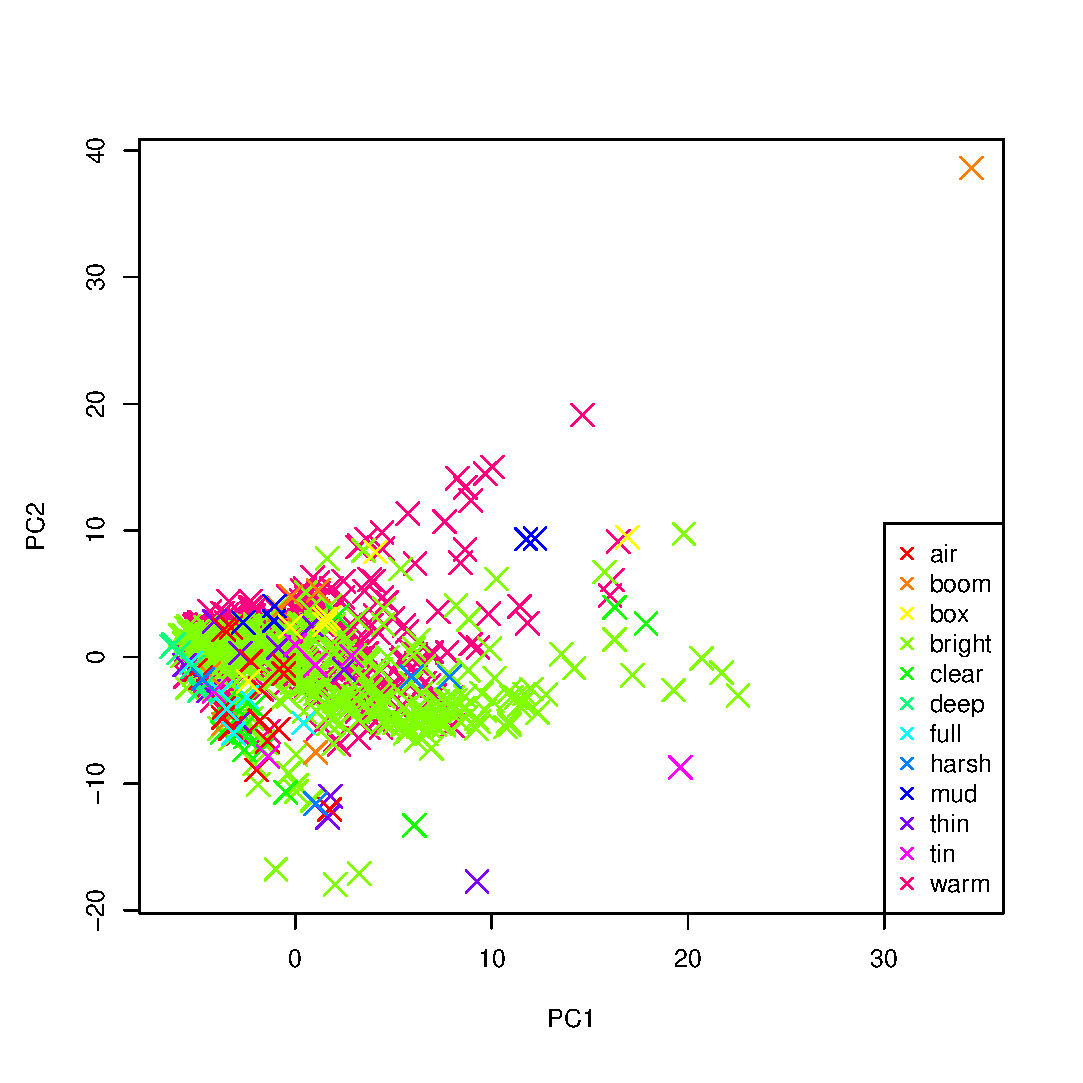
\includegraphics[width=0.45\textwidth]{chapter4/Images/EqualiserProcessedPCA.eps}
				\label{fig:EqualiserProcessedPCA}
			}
			\qquad
			\subfloat[Descriptor Centroids]
			{
				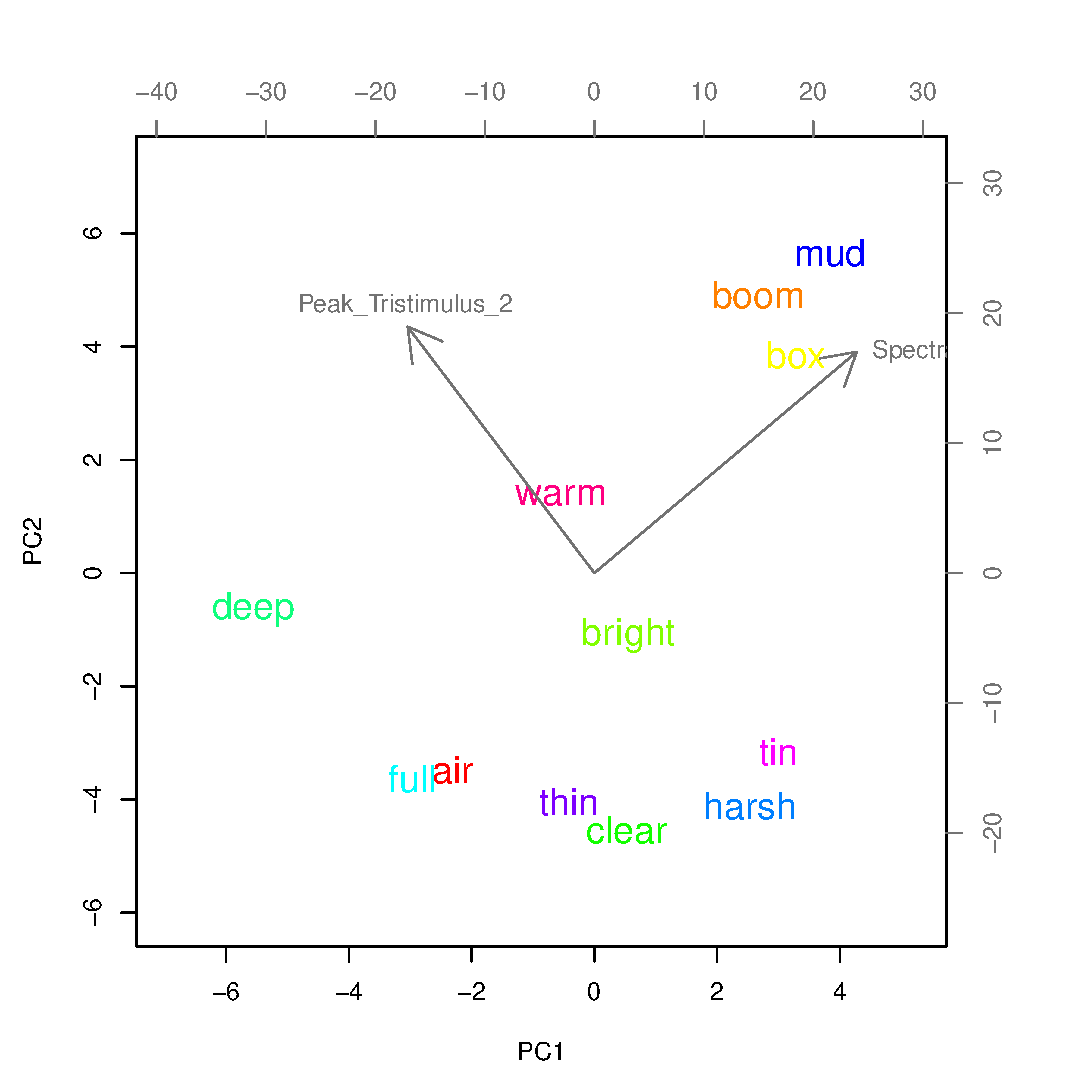
\includegraphics[width=0.45\textwidth]{chapter4/Images/EqualiserProcessedCentroidsPCA.eps}
				\label{fig:EqualiserProcessedCentroidsPCA}
			}
			\caption{Timbre space for the processed features from the equaliser.}
			\label{fig:EqualiserProcessedPCAs}
		\end{figure}

		\begin{table}
			\centering
			\begin{tabular}{|c|c|c|c|c|c|}
				\cline{2-6}
				\multicolumn{1}{c|}{} & \multicolumn{5}{c|}{\bf{Correlation}} \tabularnewline
				\hline
				\bf{Feature} & \bf{PC1} & \bf{PC2} & \bf{PC3} & \bf{PC4} & \bf{PC5} \tabularnewline
				\hline
				\hline
				\bf{Krimphoff Irregularity} & \bf{0.93} & 0.317 & 0.0106 & 0.00983 & 0.127 \tabularnewline
				\hline
				\bf{Peak Krimphoff Irregularity} & \bf{0.925} & 0.232 & 0.0194 & -0.00918 & 0.175 \tabularnewline
				\hline
				\bf{Harmonic Krimphoff Irregularity} & \bf{0.919} & 0.126 & 0.0386 & -0.0526 & 0.222 \tabularnewline
				\hline
				\bf{MFCC 10} & -0.143 & 0.00804 & \bf{-0.882} & -0.00364 & 0.0446 \tabularnewline
				\hline
				\bf{MFCC 9} & 0.0592 & -0.166 & \bf{-0.876} & -0.11 & 0.133 \tabularnewline
				\hline
				\bf{MFCC 12} & -0.069 & -0.057 & \bf{-0.867} & -0.0409 & 0.143 \tabularnewline
				\hline
				\bf{Harmonic Spectral Kurtosis} & \bf{0.862} & 0.361 & -0.0168 & -0.00383 & 0.0781 \tabularnewline
				\hline
				\bf{MFCC 8} & -0.281 & -0.0587 & \bf{-0.839} & 0.0935 & -0.14 \tabularnewline
				\hline
				\bf{Spectral Flatness} & -0.000139 & -0.223 & \bf{-0.837} & 0.0876 & 0.178 \tabularnewline
				\hline
				\bf{MFCC 11} & 0.0922 & -0.178 & \bf{-0.819} & -0.116 & 0.248 \tabularnewline
				\hline
			\end{tabular}
			\caption{Correlations between audio features and principal components for Figure
				 \ref{fig:EqualiserProcessedPCAs}}
			\label{fig:EqualiserProcessedCorrelations}
		\end{table}

		\begin{figure}[h!]
			\centering
			\subfloat[Individual Transforms]
			{
				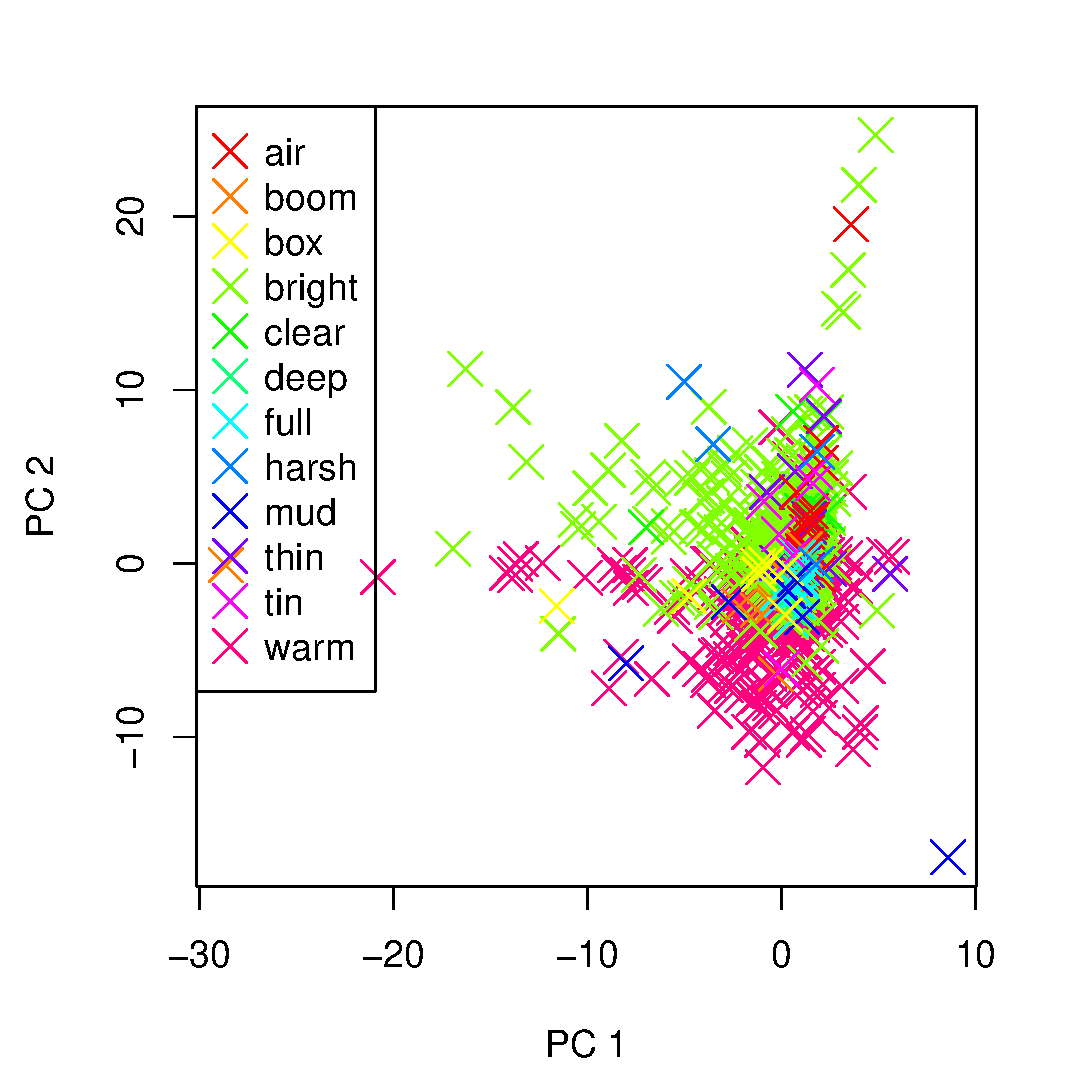
\includegraphics[width=0.45\textwidth]{chapter4/Images/EqualiserDifferencePCA.eps}
				\label{fig:EqualiserDifferencePCA}
			}
			\qquad
			\subfloat[Descriptor Centroids]
			{
				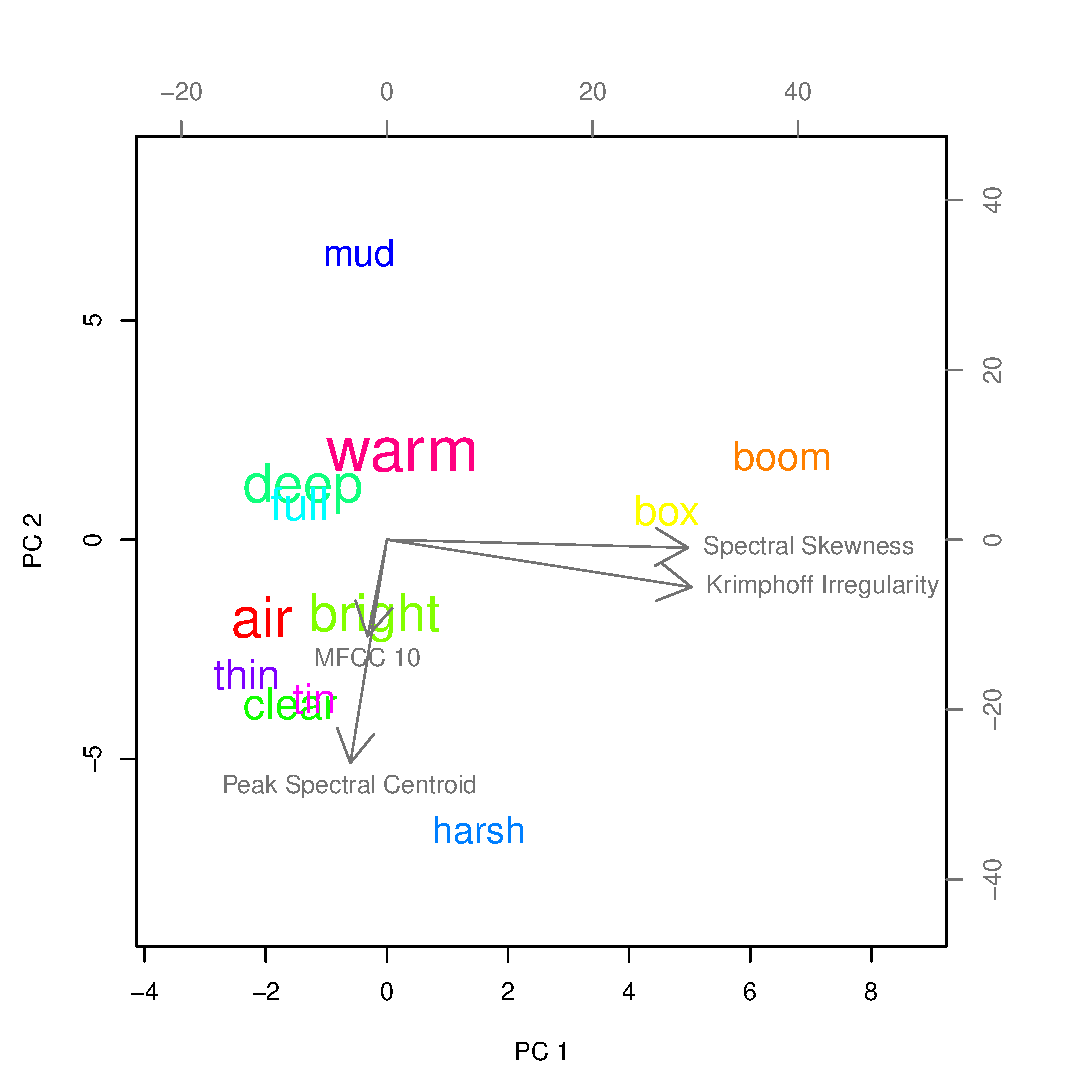
\includegraphics[width=0.45\textwidth]{chapter4/Images/EqualiserDifferenceCentroidsPCA.eps}
				\label{fig:EqualiserDifferenceCentroidsPCA}
			}
			\caption{Timbre space for the feature differences from the equaliser.}
			\label{fig:EqualiserDifferencePCAs}
		\end{figure}

		\begin{table}
			\centering
			\begin{tabular}{|c|c|c|c|c|c|}
				\cline{2-6}
				\multicolumn{1}{c|}{} & \multicolumn{5}{c|}{\bf{Correlation}} \tabularnewline
				\hline
				\bf{Feature} & \bf{PC1} & \bf{PC2} & \bf{PC3} & \bf{PC4} & \bf{PC5} \tabularnewline
				\hline
				\hline
				\bf{Krimphoff Irregularity} & \bf{0.968} & -0.182 & 0.0148 & -0.0257 & -0.0661 \tabularnewline
				\hline
				\bf{Spectral Skewness} & \bf{0.957} & -0.0311 & -0.0624 & -0.0487 & 0.108 \tabularnewline
				\hline
				\bf{Spectral Kurtosis} & \bf{0.927} & -0.0675 & -0.0408 & -0.0125 & 0.0914 \tabularnewline
				\hline
				\bf{Peak Krimphoff Irregularity} & \bf{0.892} & -0.299 & 0.0921 & 0.0312 & -0.087 \tabularnewline
				\hline
				\bf{Harmonic Spectral Kurtosis} & \bf{0.88} & -0.0525 & -0.0332 & 0.0435 & -0.0774 \tabularnewline
				\hline
				\bf{MFCC 10} & -0.0613 & -0.371 & \bf{-0.859} & 0.222 & -0.07 \tabularnewline
				\hline
				\bf{MFCC 3} & 0.0071 & 0.246 & \bf{0.859} & -0.156 & -0.03 \tabularnewline
				\hline
				\bf{Peak Spectral Centroid} & -0.116 & \bf{-0.858} & 0.219 & -0.254 & 0.0471 \tabularnewline
				\hline
				\bf{Harmonic Spectral Centroid} & -0.112 & \bf{-0.856} & 0.216 & -0.256 & 0.0369 \tabularnewline
				\hline
				\bf{MFCC 8} & -0.0488 & -0.333 & \bf{-0.851} & 0.239 & -0.0904 \tabularnewline
				\hline
				\bf{MFCC 5} & 0.102 & 0.224 & \bf{0.846} & -0.116 & 0.136 \tabularnewline
				\hline
				\bf{Peak Spectral Kurtosis} & \bf{0.845} & 0.114 & -0.136 & -0.0296 & -0.0997 \tabularnewline
				\hline
				\bf{Signal Standard Deviation} & \bf{0.844} & 0.102 & -0.15 & -0.309 & 0.114 \tabularnewline
				\hline
				\bf{RMS Amplitude} & \bf{0.844} & 0.102 & -0.15 & -0.309 & 0.114 \tabularnewline
				\hline
				\bf{MFCC 9} & -0.0745 & -0.4 & \bf{-0.842} & 0.234 & -0.0575 \tabularnewline
				\hline
				\bf{MFCC 12} & -0.0705 & -0.391 & \bf{-0.839} & 0.241 & -0.068 \tabularnewline
				\hline
				\bf{MFCC 11} & -0.0769 & -0.406 & \bf{-0.838} & 0.223 & -0.0747 \tabularnewline
				\hline
				\bf{Harmonic Krimphoff Irregularity} & \bf{0.818} & -0.392 & 0.159 & 0.0835 & -0.112 \tabularnewline
				\hline
				\bf{Harmonic Spectral Standard Deviation} & -0.23 & \bf{-0.813} & 0.146 & -0.334 & 0.205 \tabularnewline
				\hline
				\bf{Spectral Roll Off} & -0.146 & \bf{-0.804} & 0.239 & -0.282 & 0.0105 \tabularnewline
				\hline
				\bf{MFCC 4} & 0.105 & 0.379 & \bf{0.804} & -0.172 & 0.0704 \tabularnewline
				\hline
				\bf{Peak Spectral Standard Deviation} & -0.234 & \bf{-0.803} & 0.14 & -0.337 & 0.208 \tabularnewline
				\hline
			\end{tabular}
			\caption{Correlations between audio features and principal components for Figure
				 \ref{fig:EqualiserDifferencePCAs}}
			\label{fig:EqualiserDifferenceCorrelations}
		\end{table}
